%%%%%%%%%%%%%%%%%%%% author.tex %%%%%%%%%%%%%%%%%%%%%%%%%%%%%%%%%%%
%
% sample root file for your "contribution" to a contributed volume
%
% Use this file as a template for your own input.
%
%%%%%%%%%%%%%%%% Springer %%%%%%%%%%%%%%%%%%%%%%%%%%%%%%%%%%


% RECOMMENDED %%%%%%%%%%%%%%%%%%%%%%%%%%%%%%%%%%%%%%%%%%%%%%%%%%%
\documentclass[graybox]{svmult}

% choose options for [] as required from the list
% in the Reference Guide

\usepackage{type1cm}        % activate if the above 3 fonts are
                            % not available on your system
%
\usepackage{makeidx}         % allows index generation
\usepackage{graphicx}        % standard LaTeX graphics tool
                             % when including figure files
\usepackage{multicol}        % used for the two-column index
\usepackage[bottom]{footmisc}% places footnotes at page bottom


\usepackage{newtxtext}       % 
\usepackage[varvw]{newtxmath}       % selects Times Roman as basic font

% see the list of further useful packages
% in the Reference Guide

\makeindex             % used for the subject index
                       % please use the style svind.ist with
                       % your makeindex program

%%%%%%%%%%%%%%%%%%%%%%%%%%%%%%%%%%%%%%%%%%%%%%%%%%%%%%%%%%%%%%%%%%%%%%%%%%%%%%%%%%%%%%%%%

\begin{document}

\title*{A cloud-native data science platform to build production-grade machine learning systems}
\titlerunning{A cloud-native data science platform to build production-grade ML systems}
\author{Romain Avouac and\\ Thomas Faria and\\ Frédéric Comte}
\institute{Romain Avouac 
\at Insee (National Institute of Statistics and Economic Studies), 
\email{romain.avouac@insee.fr}
\and Thomas Faria 
\at Insee (National Institute of Statistics and Economic Studies), 
\email{thomas.faria@insee.fr}
\and Frédéric Comte 
\at Insee (National Institute of Statistics and Economic Studies), 
\email{frederic.comte@insee.fr}}

\maketitle

\abstract*{In recent years, statisticians trained in data science methods have been joining National Statistical Offices (NSOs), aiming to harness non-traditional data sources and machine learning methods to enhance the production of official statistics. Despite their expertise, these professionals encounter significant barriers, including limited computational resources, inflexible development environments that do not foster collaborative work, and limited tools to transition from innovative experiments to production-grade solutions. This paper presents Onyxia, an open-source project developed to address these challenges by enabling organizations to build modern and flexible data science environments that enhance the autonomy of statisticians. With Onyxia and its showcase instance, the SSP Cloud, we demonstrate how cloud technologies can be made readily accessible, fostering innovation, collaboration and reproducibility in the field of official statistics. Through a case study of the classification of the activity domain (NACE) of French companies, we illustrate how these tools have been instrumental in operationalizing machine learning models in accordance with MLOps principles, marking a significant step forward in the valorisation of data science projects at Insee.}

\abstract{In recent years, statisticians trained in data science methods have been joining National Statistical Offices (NSOs), aiming to harness non-traditional data sources and machine learning methods to enhance the production of official statistics. Despite their expertise, these professionals encounter significant barriers, including limited computational resources, inflexible development environments that do not foster collaborative work, and limited tools to transition from innovative experiments to production-grade solutions. This paper presents Onyxia, an open-source project developed to address these challenges by enabling organizations to build modern and flexible data science environments that enhance the autonomy of statisticians. With Onyxia and its showcase instance, the SSP Cloud, we demonstrate how cloud technologies can be made readily accessible, fostering innovation, collaboration and reproducibility in the field of official statistics. Through a case study of the classification of the activity domain (NACE) of French companies, we illustrate how these tools have been instrumental in operationalizing machine learning models in accordance with MLOps principles, marking a significant step forward in the valorisation of data science projects at Insee.}




\section{Introduction}
\label{sec:introduction}

In recent years, the European Statistical System (ESS) has committed to leverage non-traditional data sources in order to improve the process of statistical production, an evolution that is encapsulated by the concept of Trusted Smart Statistics \cite{ricciato2019trusted}. This dynamic is accompanied by innovations in the statistical processes, so as to be able to take advantage of the great potential of these new sources (greater timeliness, increased spatio-temporal resolution, etc.), but also to cope with their complexity or imperfections. At the forefront of these innovations are machine-learning methods and their promising uses in the coding and classification fields, data editing and imputation \cite{gjaltema2022high}. The multiple challenges faced by statistical offices because of this evolution are addressed in the Bucharest Memorandum on Official Statistics in a Datafied Society (Trusted Smart Statistics), which predicts that "the variety of new data sources, computational paradigms and tools will require amendments to the statistical business architecture, processes, production models, IT infrastructures, methodological and quality frameworks, and the corresponding governance structures", and consequently invites the ESS to assess the required adaptations and prioritize them \cite{bucharest2018}.

In line with these recommendations, much work has been done in the context of successive projects at the European level in order to operationalize the use of non-traditional data sources in the production of official statistics. Within the scope of the ESSnet Big Data II project (2018-2020), National Statistical Offices (NSOs) have been working across a wide range of themes (online job vacancies, smart energy, tracking ships, etc.) in order to put together the building blocks for using these sources in actual production processes and identify their limitations \cite{essnetbigdata2}. However, while a substantial amount of work has been devoted to developing methodological frameworks \cite{descy2019towards, salgado2020mobile}, quality guidelines \cite{kowarik2022quality} as well as devising business architectures that make third-party data acquisition more secure \cite{ricciato2018processing}, not much has been said about the IT infrastructures and skills needed to properly deal with these new objects.

The characteristics of big data sources make them particularly complex to process, be it their volume, their velocity (speed of creation or renewal) or their variety (structured but also unstructured data, such as text and images). Besides, the "skills and competencies to automate, analyse, and optimize such complex systems are often not part of the traditional skill set of most National Statistical Offices" \cite{ashofteh2021data}. Not incidentally, an increasing number of public statisticians trained as data scientists have joined NSOs in recent years. Within its multiple meanings, the term “data scientist” reflects the increased involvement of statisticians in the IT development and orchestration of their data processing operations, beyond merely the design or validation phases \cite{davenport2012data}. However, based on our observations at Insee and other French statistical offices, the ability of these new data professionals to derive value from big data sources and machine learning methods is limited by several challenges.

A first challenge is related to the lack of proper IT infrastructures to tackle the new data sources that NSOs now have access to as well as the accompanying need for new statistical methods. For instance, big data sources require huge storage capacities and often rely on distributed computing frameworks to be processed \cite{liu2013computing}. Similarly, the adoption of new statistical methods based on machine learning algorithms often requires IT capacities — in particular, GPUs (graphical processing units) — to massively parallelize computations \cite{saiyeda2017cloud}. Such resources are not readily available in traditional IT infrastructures. Furthermore, these new infrastructures generally require specific skills — especially to build and maintain them — that are not easily found in NSOs.

Another major challenge lies in equipping statisticians with development environments that enable them to experiment more freely. The essence of innovation in statistical work lies in the ability to swiftly adapt to and incorporate new tools and methodologies. This agility is hampered when statisticians depend excessively on IT departments to provision resources or install new software packages. In traditional setups — personal computers or virtual desktops on centralized architectures — IT departments generally prioritize security and system stability over the provision of new services, which limits the innovation potential. Besides, these rigid environments make it harder to implement development best practices, such as collaborative work — which requires environments where experiments can be easily shared with peers — and reproducibility.

A third challenge is related to the difficulty of transitioning from innovative experiments to production-grade solutions. Even when statisticians have access to development environments in which they can readily experiment, the step towards deploying an application or a model is generally very large. Production environments often differ from development environments in such a way that the additional development costs needed to go from a proof of concept to an industrialized solution that actually serves users can limit the feasibility of this transition. Furthermore, in the case of machine learning projects, models that have been deployed require a proper monitoring to ensure that they maintain their accuracy and utility over time, and generally require periodic or continuous improvements. Again, this pleads for more flexible environments that enable statisticians to manage the complete lifecycle of their data science projects in a more continuous way.

We argue that these various challenges have an underlying common theme: the need for more autonomy. The ability of data science methods to improve and potentially transform the production of official statistics crucially depends on the ability of statisticians to carry out innovative experiments more freely. To do so, they need to have access to substantial and diverse computing resources that enable them to tackle the volume and diversity of big data sources and leverage machine learning methods. Such experimental projects require, in turn, flexible development environments that foster collaborative work in order to capitalize the diversity of profiles and skills that compose project teams. Finally, to derive value from these experiments, statisticians require tools to deploy applications as proof-of-concepts and orchestrate their statistical operations autonomously.

Against this background, Insee developed Onyxia: an open source project that enables organizations to deploy data science platforms that foster innovation by giving statisticians more autonomy\footnote{\url{https://github.com/InseeFrLab/onyxia}}. This paper aims at describing the full thought process that led to this project and at exemplifying how it empowers statisticians at Insee, thus becoming a cornerstone of our innovation strategy. Section~\ref{sec:principles} provides an in-depth analysis of the data ecosystem's latest developments, casting light on the technological choices that have shaped the development of a modern data science environment tailored to the specific needs of statisticians. In particular, we show how cloud-native technologies — particularly containers and object storage — are key to building scalable and flexible environments that can enhance autonomy while promoting reproducibility in the production of official statistics. However, despite their appealing attributes for modern data science applications, the complexity of configuring and utilizing cloud technologies often poses barriers to their broad adoption. In section~\ref{sec:implementation}, we detail the core of the Onyxia project: how we made cloud technologies accessible to statisticians through a user-friendly interface and an extensive catalogue of ready-to-use data science environments, while circumventing potential vendor lock-in effects for both the institution and their users. We also show how providing an open-innovation instance of Onyxia, the SSP Cloud, greatly facilitated the adoption of these technologies and fostered improved development practices. Finally, through the case study of the classification of French companies' activity (NACE), section~\ref{sec:mlops} illustrates how leveraging these technologies greatly facilitated the deployment of machine learning models at Insee in alignment with the industry best practices — namely, MLOps principles.




\section{Principles for building a modern and flexible data architecture for official statistics}
\label{sec:principles}

With the emergence of big data sources and new methodologies offering significant promise to improve the production process of official statistics, statisticians trained in data science techniques are eager to innovate. However, their ability to do so is limited by several challenges. Central among these challenges is the need for greater autonomy — be it in scaling resources to match statistical workloads, deploying proofs of concept with agility and in a collaborative manner, etc. Against this background, our aim was to design a data science platform that not only manages big data efficiently but also empowers statisticians by enhancing their autonomy. To achieve this, we looked at the evolution of the data ecosystem to identify significant trends that could help overcome the above-mentioned limitations\footnote{As a preamble to this review, we should note that, although we did our best to ground our insights in the academic literature, a lot of it stems from informal knowledge  gathered through diligent and ongoing technology watch. In the rapidly evolving data ecosystem, traditional research papers are increasingly giving way to blog posts as the primary references for cutting-edge developments. This shift is largely due to the swift pace at which big data technologies and methodologies are advancing, making the lengthy publication process of formal research often not the preferred way of disseminating timely insights and innovations.}. Our findings indicate that leveraging cloud-native technologies, particularly containers and object storage, is key to building infrastructures capable of handling large and varied datasets in a flexible and cost-effective manner. Furthermore, these technologies significantly enhance autonomy, facilitating innovation and promoting reproducibility in the production of official statistics.

\subsection{Limitations of traditional big data architectures}

Over the last decade, the landscape of big data has dramatically transformed. Following the publication of Google's seminal papers that introduced the MapReduce paradigm \cite{ghemawat2003google, dean2008mapreduce}, Hadoop-based systems rapidly became the reference architecture of the big data ecosystem, celebrated for their capability to manage extensive datasets through the use of distributed computing. The introduction of Hadoop marked a revolutionary step, enabling organizations to process and analyse data at an unprecedented scale. Basically, Hadoop provided companies with all-rounded capabilities for big data analytics: tools for ingestion, data storage (HDFS), and computing capacities (Spark, among others) \cite{dhyani2014big}, thus explaining its rapid adoption across industries.

In the late 2010s, Hadoop-based architectures have experienced a clear decline in popularity. In traditional Hadoop environments, storage and compute were co-localized by design: if the source data is distributed across multiple servers (horizontal scaling), each section of the data is directly processed on the machine hosting that section, so as to avoid network transitions between servers. In this paradigm, scaling the architecture often meant a linear increase in both compute and storage, regardless of the actual demand. In a recent article provocatively titled "Big Data is Dead"\footnote{\url{https://motherduck.com/blog/big-data-is-dead/}}, Jordan Tigani, one of the founding engineers behind Google BigQuery, explains why this model does not fit the reality of most data-centric organizations anymore. First, because "in practice data sizes increase much faster than compute sizes". While the amount of data generated and thus needing to be stored may grow linearly over time, it is generally the case that we only need to query the most recent portions of it, or only some columns and/or groups of rows. Besides, Tigani points out that "the big data frontier keeps receding": advancements in server computing capabilities and declining hardware costs mean that the number of workloads that do not fit on a single machine — a simple yet effective definition of big data — has been continually decreasing. As a result, by properly separating storage and compute functions, even substantial data processing jobs may end up using "far less compute than anticipated [...] and might not even need to use distributed processing at all".

These insights strongly align with our own observations at Insee in recent years. For instance, an Insee team set up a Hadoop cluster as an alternative architecture to the one already in use to process sales receipt data in the context of computing the consumer price index. An acceleration of data processing operations by up to a factor of 10 was achieved, for operations that previously took several hours to perform \cite{leclair2019utiliser}. Despite this increase in performance, this type of architectures were not reused later for other projects, mainly because the architecture proved to be expensive and complex to maintain, necessitating specialized technical expertise rarely found within NSOs \cite{vale2015international}. Although these new projects could still involve substantial data volumes, we observed that effective processing could be achieved using conventional software tools (R, Python) on single-node systems by leveraging recent important innovations from the data ecosystem. First, by using efficient formats to store the data such as Apache Parquet \cite{parquet2013}, which properties — columnar storage \cite{abadi2013design} (see figure\ref{fig:columnar-storage}), optimization for "write once, read many" analytics, ability to partition data, etc. — make it particularly suited to analytical tasks such as those generally performed in official statistics \cite{abdelaziz2023optimizing}. Second, by performing computations using optimized in-memory computation frameworks such as Apache Arrow \cite{arrow2016} or DuckDB \cite{raasveldt2019duckdb}. Also based on columnar representation — thus working in synergy with Parquet files — both of these frameworks greatly improve data queries performance through the use of "lazy evaluation": instead of doing lots of separate operations (e.g. selecting columns and/or filtering rows, then computing new columns, then performing aggregations, etc.), they process them all at once in a more optimized way. As a result, computations are limited to the data effectively needed by the queries, enabling much larger-than-memory data processing on usual single-node machines.

\begin{figure}[htbp]
    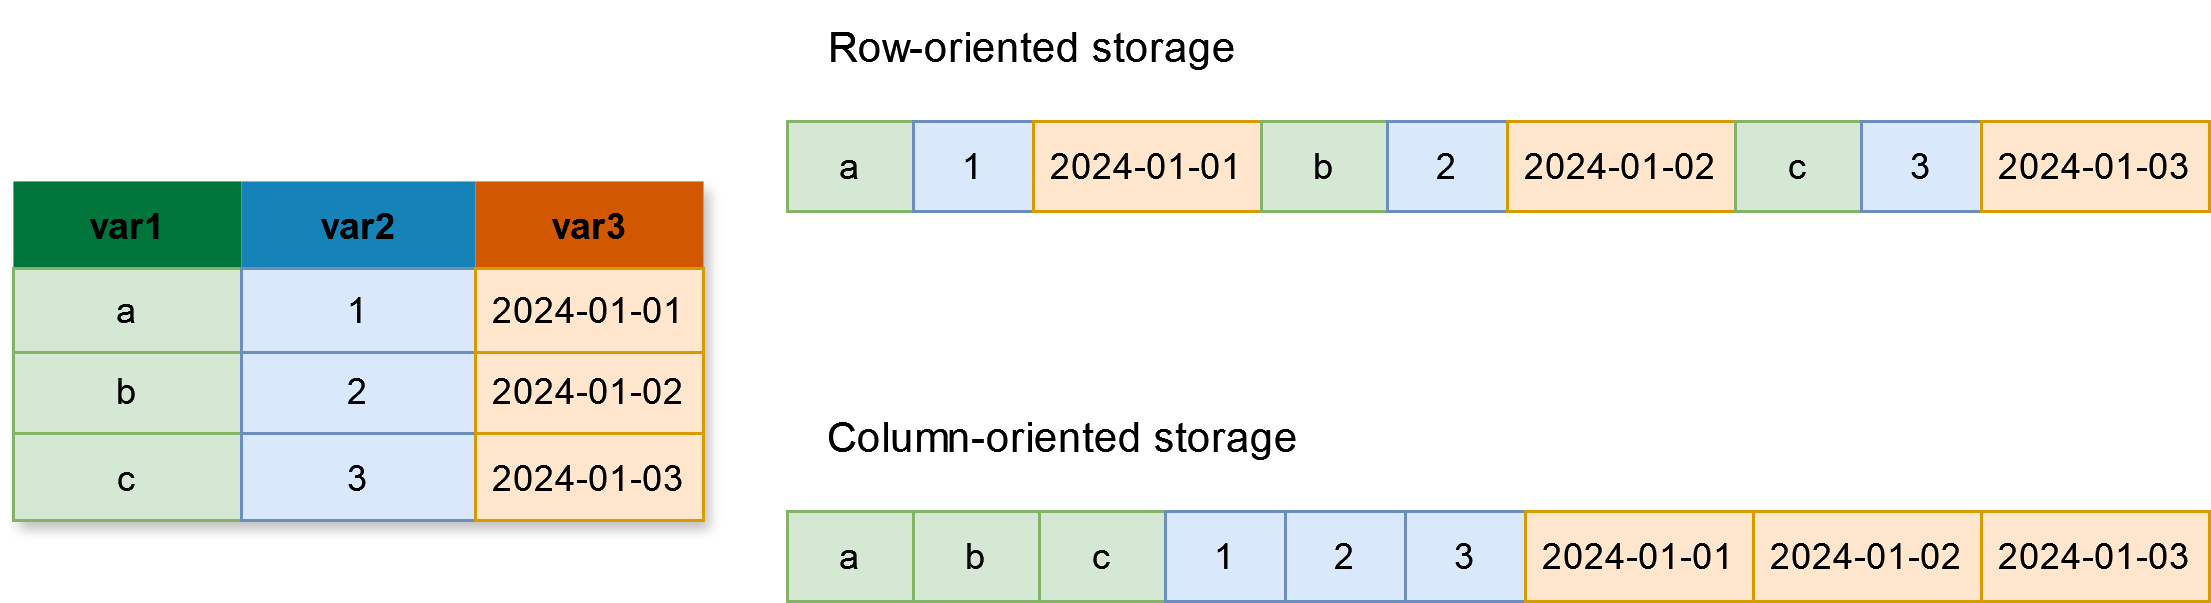
\includegraphics[width=\linewidth]{figures/columnar-storage.png}
    \caption{Row-oriented and column-oriented representation of a same dataset.}
    \label{fig:columnar-storage}
    \medskip
    {\footnotesize Note: Many statistical operations are analytical (OLAP) in nature: they involve selecting specific columns, computing new variables, performing group-based aggregations, etc. Row-oriented storage is not well-suited to analytical operations as it requires the full dataset to be read in memory to query it. Conversely, column-based storage allows only relevant data columns to be queried, significantly reducing read and processing times for analytical workloads. In practice, popular columnar formats such as Parquet use a hybrid-representation: they are primarily column-oriented but also implement clever row-based grouping to optimize filtering queries.}
\end{figure}

\subsection{Embracing cloud-native technologies}
\label{sec:cloud-native}

In light of this evolution of the big data ecosystem, there has been a notable shift in recent years within the industry towards more flexible and loosely coupled architectures. The advent of cloud technologies has been instrumental in facilitating this shift. Unlike the era where Hadoop was prominent, network latency has become much less of a concern, making the traditional model of on-premise and co-located storage and compute solutions less relevant. Regarding the nature of the data that needs to be processed, we observe an evolution that some have described as moving "from big data to flexible data". Modern data infrastructures are required not only to process large volumes but also to be adaptable in multiple dimensions. They must accommodate various data structures (ranging from structured, tabular formats to unstructured formats like text and images), ensure data portability across multi-cloud and hybrid cloud environments, and support a diverse range of computational workloads (from parallel computations to deep learning models necessitating GPUs, as well as the deployment and management of applications) \cite{li2020big}. In recent years, two technologies have emerged in the data ecosystem as foundational technologies for achieving such flexibility in cloud-based environments: containerization and object storage. 

In a cloud environment, the computer of the user becomes a simple access point to perform computations on a central infrastructure. This enables both ubiquitous access to and scalability of the services, as it is easier to scale a central infrastructure — usually horizontally, i.e. by adding more servers. However, such centralized infrastructures have two well-identified limitations that need to be dealt with: the competition between users in access to physical resources and the need to properly isolate deployed applications. The choice of containerization is fundamental as it tackles these two issues \cite{bentaleb2022containerization}. By creating “bubbles” specific to each service, containers guarantee application isolation while remaining lightweight, as they share the support operating system with the host machine (see. graph~\ref{fig:containers}). In order to manage multiple containerized applications in a systematic way, containerized infrastructures generally rely on an orchestrator software — the most prominent one being Kubernetes, an open-source project initially developed by Google to manage its numerous containerized workloads in production \cite{vano2023cloud}. Orchestrators automate the process of deploying, scaling, and managing containerized applications, coordinating their execution across various servers. Interestingly, this property makes it possible to handle very large volumes of data in a distributed way: containers break down big data processing operations into a multitude of small tasks, organized by the orchestrator. This minimizes the required resources while providing more flexibility than Hadoop-based architectures \cite{zhang2018comparative}.

\begin{figure}[htbp]
    \begin{center}
        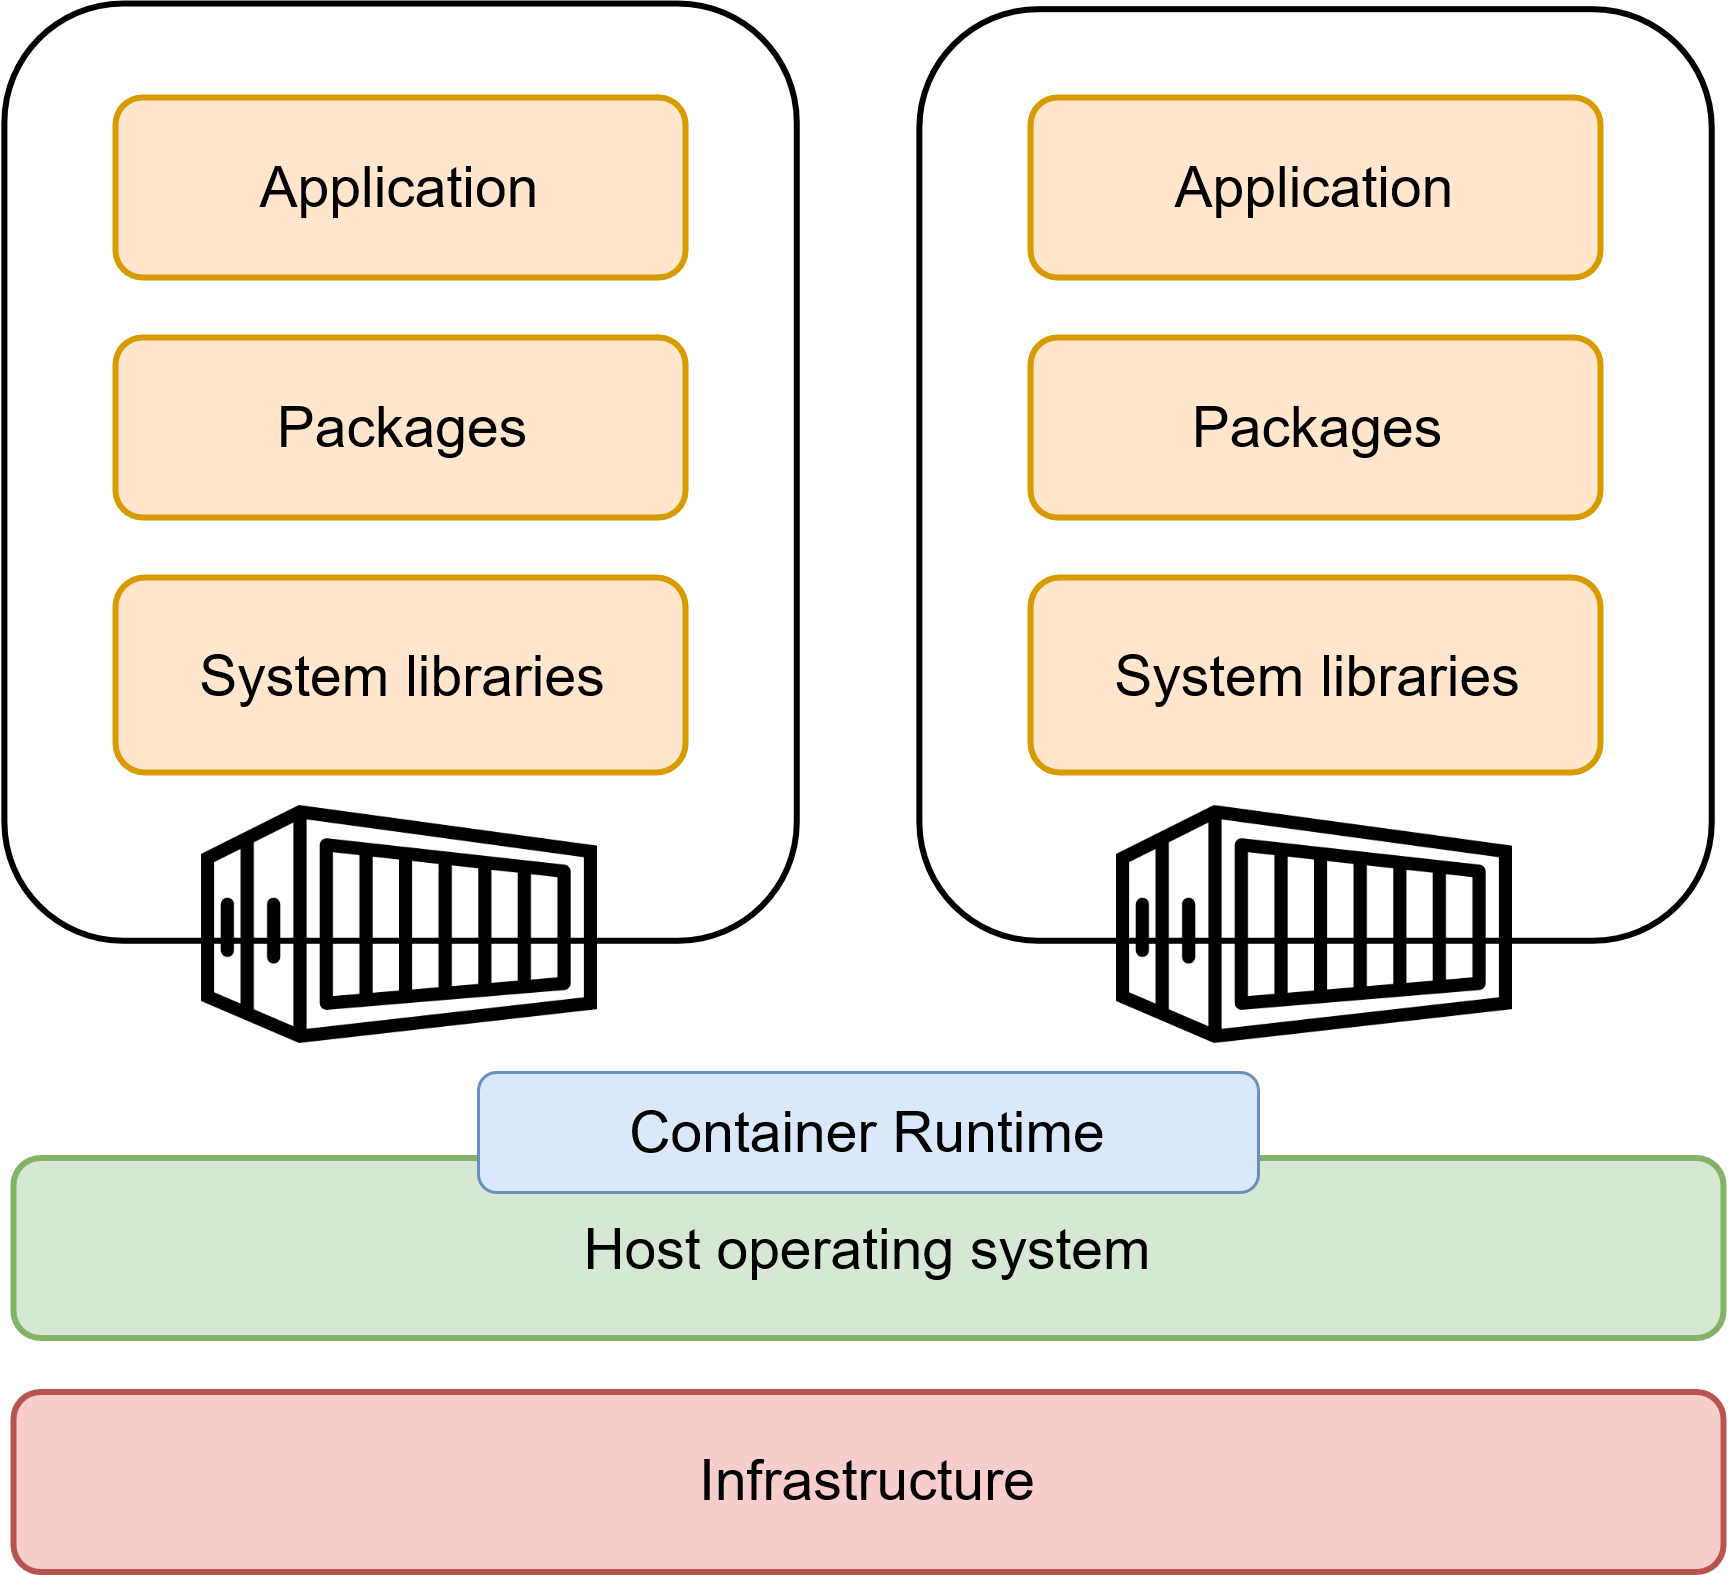
\includegraphics[width=0.65\linewidth]{figures/containers.png}
    \end{center}
    \caption{Architecture of a containerized environment.}
    \label{fig:containers}
    \medskip
    {\footnotesize Note: A container is a logical grouping of resources that makes it possible to encapsulate an application (e.g. Python code), the packages used (e.g. Pandas, NumPy) and system libraries (the Python interpreter, other OS-dependent libraries, etc.), in a single package. Containerized applications are isolated from one another through virtualization, which makes it possible to attribute specific physical resources to each application while guaranteeing complete independence between them. But contrary to virtual machines which also virtualize the operating system (OS), containers rely on a lightweight form of virtualization: the container shares the OS of the host infrastructure through the container runtime (e.g. Docker). As a result, containers are much more portable and can be readily deployed and redistributed.}
\end{figure}

The other fundamental choice in a data architecture is the nature of data storage. In the cloud ecosystem, so-called "object storage" has become the {\it de facto} reference \cite{samundiswary2017object}\footnote{Mainly because of Amazon's "S3" (Simple Storage Service) implementation.}. In this paradigm, files are stored as "objects" consisting of data, an identifier and metadata. This type of storage is optimized for scalability, as objects are not limited in size and the underlying technology enables cost-effective storage of (potentially very) large files. It is also instrumental in building a decoupled infrastructure such as discussed before: the data repositories — referred to as "buckets" — are directly searchable using standard HTTP requests through a standardized REST API. In a world where network latency is not the main bottleneck anymore, this means that storage and compute do not have to be on the same machines or even in the same location, and can thus scale independently according to specific organization demands. Finally, object storage is a natural complement to architectures based on containerized environments for which it provides a persistence layer — containers being stateless by design — and easy connectivity without compromising security, or even with strengthened security compared with a traditional storage system \cite{mesnier2003object}.

\subsection{Leveraging cloud technologies to increase autonomy and foster reproducibility}

Understanding how the technological choices described in the technical discussion above are relevant in the context of official statistics require an in-depth review of statisticians’ professional practices in their use of computing environments. At the end of the 2000s, with microcomputing at its peak, many of the technical resources used by statisticians at Insee were local: the code and processing software were located on personal computers, while data was accessed through a file-sharing system. Because of the limited scalability of personal computers, this setup greatly limited the ability of statisticians to experiment with big data sources or computationally intensive statistical methods, and involved security risks because of the widespread data dissemination within the organization. In order to overcome these limitations, a transition was made towards centralized IT infrastructures, concentrating all — and thus overall much more — resources on central servers. Such infrastructures, made available to statisticians through a shared, virtual desktop environment for ease of use, remains the dominant method for conducting statistical computations at Insee at the time of writing these lines.

Through our observations and discussions with fellow statisticians, it became obvious that although the current IT infrastructure adequately supported the core activities of statistical production, it noticeably restricted statisticians' capacity to experiment freely and innovate. The primary bottleneck in this organization is the dependency of statistical projects on centralized IT decision-making, such as the allocation of computing resources, access to shared data storage, the use of pre-configured programming languages and packaging environments, etc. Besides, such dependencies often lead to a well-known phenomenon within the software development community that lies at the heart of the DevOps approach, where the priorities of developers — iterate rapidly to improve functionality in a continuous manner — often clash with IT's focus on security and process stability. On the contrary, it is our understanding that modern data science practices reflect an increased involvement of statisticians in the IT development and orchestration of their data processing operations, beyond merely the design or validation phases. New data science infrastructures must take this expanded role of their users into account, giving them more autonomy than conventional infrastructures.

We argue that cloud technologies stand out as a powerful solution to give statisticians much more autonomy in their daily work, enabling a culture of innovation. Through object storage, users gain control over the storage layer, allowing them to experiment with diverse datasets without being constrained by the limited storage spaces typically allocated by IT departments. Containerization empowers users to customize their working environments to their specific needs — be it programming languages, system libraries, or package versions — while also providing the flexibility to scale their applications according to the required computing power and storage capacities. By design, containers also foster the development of portable applications, which enables smoother transitions between environments (development, testing, staging, production), ensuring that applications can be moved seamlessly without the hurdles of environmental inconsistencies. Finally, with orchestration tools like Kubernetes, statisticians can more readily deploy applications and APIs and automatize the whole building process. This capability aligns with the DevOps approach, enabling quicker iteration and building minimal prototypes as proofs of concept (POCs) rather than building the optimal (but time-consuming) solution for a pre-defined objective \cite{leite2019survey}.

\begin{figure}[htbp]
    \begin{center}
        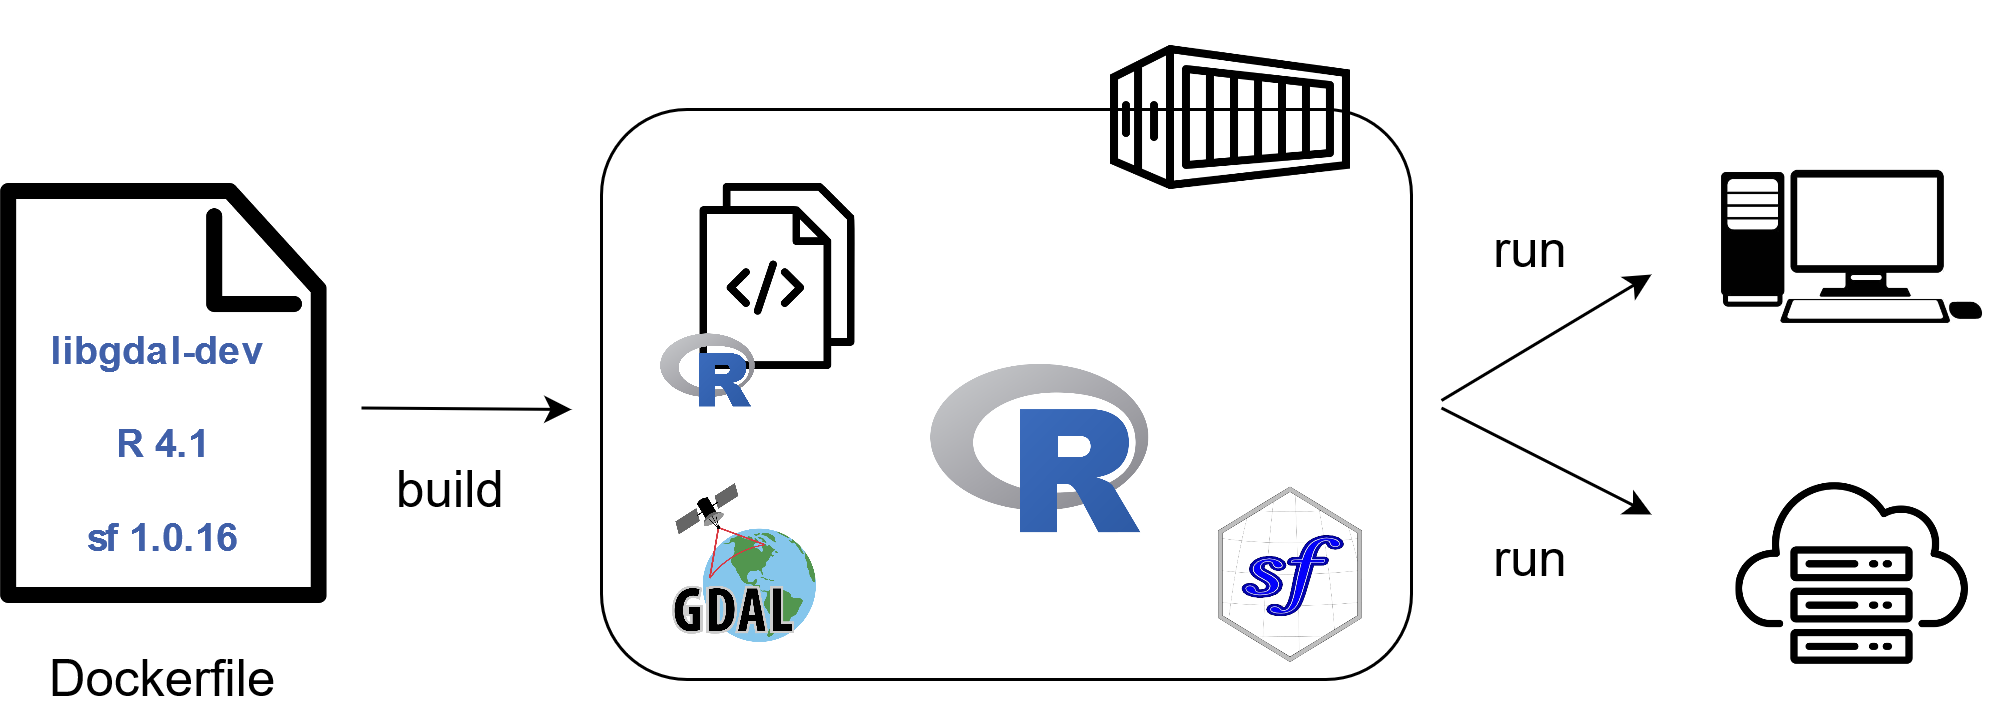
\includegraphics[width=0.85\linewidth]{figures/containers-portability.png}
    \end{center}
    \caption{Containers foster reproducibility and portability by design.}
    \label{fig:containers-portability}
    \medskip
    {\footnotesize Note: In a containerized environment, applications are created through script specifications — a paradigm known as "infrastructure as code". In a text file conventionally named "Dockerfile", data scientists can specify the working environment of their application: the application code, the software to be included (e.g. R), the packages used for their processing operations (e.g. the R package for geospatial computation \textit{sf}), and the OS-dependent system libraries that are called by these packages (e.g. GDAL, the translator library for raster geospatial data formats used by most packages dealing with geospatial data). Importantly, the versions of the software and packages that were used to develop the application can be precisely specified, which guarantees reproducibility of the computations performed. A build step then creates an image associated to the Dockerfile, i.e. a packaged and compressed form of the working environment of the application. Images created this way are portable: they can be readily distributed — usually through a container registry — and executed in a reproducible manner on any infrastructure that has a container runtime. 
    }
\end{figure}

Besides scalability and autonomy, these architectural choices also foster reproducibility of statistical computations. The concept of reproducibility — namely the ability to reproduce the result of an experiment by applying the same methodology to the same data — is a fundamental criterion of scientific validity \cite{mcnutt2014reproducibility}. It is also highly relevant in official statistics, as it serves as a foundation for transparency, which in turn is crucial for building and maintaining the public's trust \cite{eurocodepractice2018}. Fostering reproducibility in statistical production involves devising processing solutions that can produce reproducible statistics on the one hand, and that can be shared with peers on the other hand \cite{ntts2019reproducibility}. Traditional IT infrastructures — either a personal computer or a shared infrastructure with remote desktop access — fall short in this regard, as building a project or just computing a statistical indicator there generally involves a series of manual steps (installing system libraries, the programming language binary, projects packages, dealing with potentially conflicting versions, etc.) that can not be fully reproduced across projects. In comparison, containers are reproducible by design, as their build process involves defining precisely all the needed resources as a set of processing operations in a standardized manner, from the "bare machine" to the running application \cite{moreau2023containers}. Furthermore, these reproducible environments can be easily shared to peers as they can be readily published on open registries (for example, a container registry such as DockerHub) along with the source code of the application (for example, on a public software forge like GitHub or GitLab). This approach significantly enhances the re-usability of code projects, fostering a community-driven model of development and innovation.




\section{Onyxia: an open source project to build cloud-native data science platforms}
\label{sec:implementation}

This section explores how Onyxia, an open-source project initiated at Insee, democratizes access to cloud technologies for statisticians by providing modern data science environments that foster autonomy. We discuss how this initiative fits in with the general aim of creating "knowledge commons" by promoting and building software that can be easily reused in the field of official statistics and beyond.

\subsection{Making cloud-technologies accessible to statisticians}

Our technology watch and literature review highlighted cloud-native technologies, in particular containerization and object storage, as instrumental in building a data science platform that is both scalable and flexible. Building on these insights, we established our initial on-premise Kubernetes cluster in 2020, integrating it with MinIO, an open-source object storage system designed to work seamlessly with Kubernetes. Yet, our first experiments highlighted a significant barrier to the widespread adoption of cloud-native technologies: the complexity of their integration. This is an important consideration when building data architectures that prioritize modularity — an essential feature for the flexibility we aim to achieve. For instance, due to MinIO's compatibility with the Amazon S3 API, the storage source could easily be switched to  one managed by another public cloud provider, without requiring substantial modifications. However, modularity of the architecture components also entails that any data application launched on the cluster must be configured so as to communicate with all the components. For instance, in a big data setup, configuring Spark to operate on Kubernetes while interacting with datasets stored in MinIO requires an intricate set of configurations (specifying endpoints, access tokens, etc.), a skill set that typically lies beyond the expertise of statisticians.

This insight is really the base of the Onyxia project: choosing technologies that foster autonomy will not actually foster autonomy if their complexity acts as a barrier from widespread adoption in the organization. In recent years, statisticians at Insee already needed to adapt to a changing environment in terms of their everyday tools: transitioning from proprietary software (SAS®) to open-source ones (R, Python), acculturating to technologies that improve reproducibility (version control with Git), consuming and developing APIs, etc. These changes, making their job more and more akin to the one of software developers, already imply significant training and changes in daily work practices. Against this background, adoption of cloud-technologies was utterly dependent on making them readily accessible.

\begin{figure}[htbp]
    \centering
    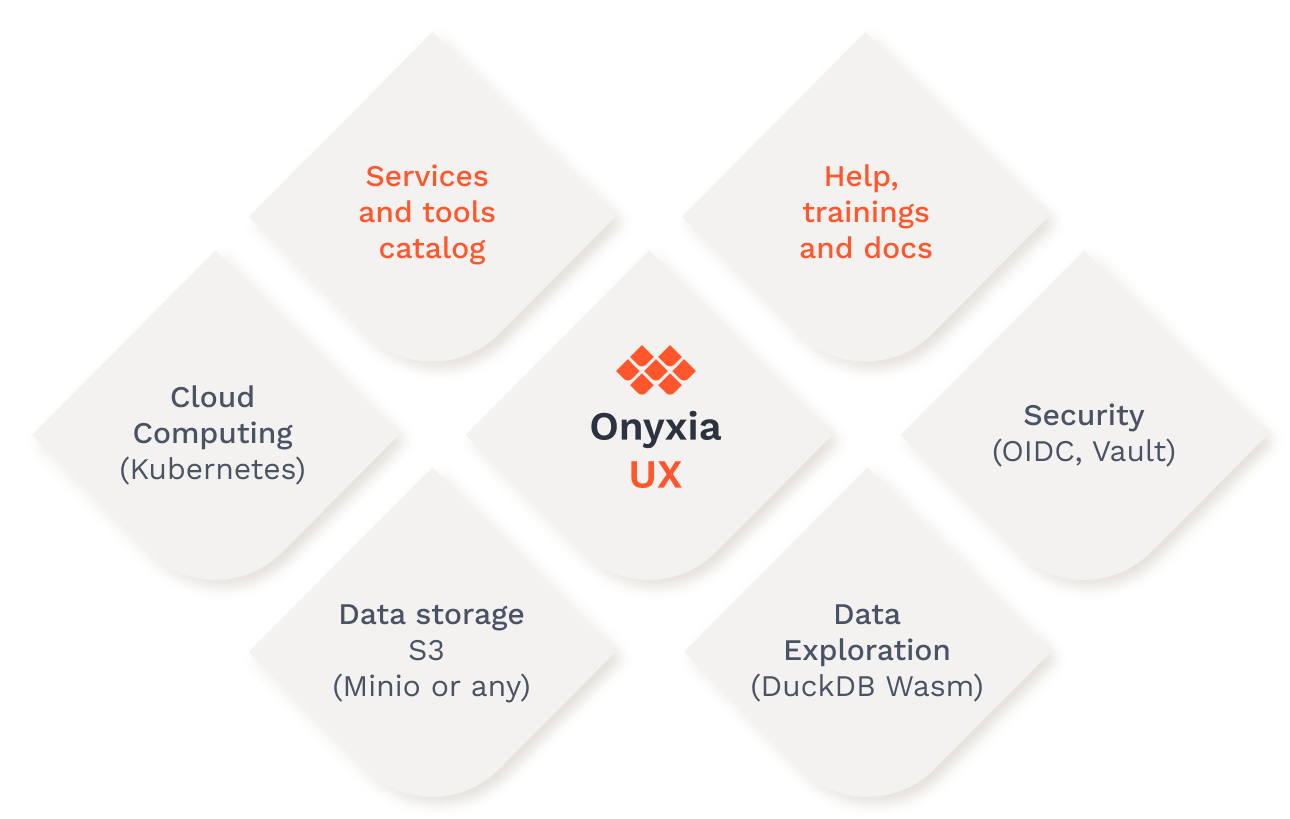
\includegraphics[width=\linewidth]{figures/onyxia-components.png}
    \caption{Onyxia is the technical binder between cloud-native modular components}
    \label{fig:onyxia-components}
\end{figure}

To bridge this gap, we developed Onyxia, an application that essentially acts as interface between the modular components that compose the architecture (see fig~\ref{fig:onyxia-components}). The main entry point of the user is a user-friendly web application\footnote{\url{https://github.com/InseeFrLab/onyxia-ui}} that enables users to launch services from a data science catalog (see section \ref{ssec:catalog}) as running containers on the underlying Kubernetes cluster. The interface between the UI and Kubernetes is done by a lightweight custom API\footnote{\url{https://github.com/InseeFrLab/onyxia-api}}, that essentially transforms the application request of the user into a set of manifests to deploy Kubernetes resources. For a given application, these resources are packaged under the form of Helm charts, a popular way of packaging potentially complex applications on Kubernetes \cite{gokhale2021creating}. Although users can configure a service to tailor it to their needs, they will most of the time just launch an out-of-the-box service with default settings and start developing straight away. This point really illustrates the added value of Onyxia in facilitating the adoption of cloud technologies. By injecting authentication information and configuration into the containers at the initialization, we ensure that users can launch and manage data science services in which they can interact seamlessly with the data from their bucket on MinIO, their sensitive information (tokens, passwords) in a secret management tool such as Vault, etc. This automatic injection, coupled with the pre-configuration of data science environments in Onyxia's catalogs of images\footnote{\url{https://github.com/InseeFrLab/images-datascience}} and associated helm-charts\footnote{\url{https://github.com/InseeFrLab/helm-charts-interactive-services}}, make it possible for users to execute potentially complex workloads — such as running distributed computations with Spark on Kubernetes using data stored in S3, or training deep-learning models using a GPU — without getting bogged down by the technicalities of configuration.

\subsection{Architectural choices aimed at fostering autonomy}
\label{ssec:principles}

The Onyxia project is based on a few structuring principles, with a central theme: fostering autonomy, both at the organizational and individual levels. First, at the level of the organization by preventing vendor lock-in. In order to get a competitive edge, many commercial cloud providers develop applications and protocols that customers need to use to access cloud resources, but that are not interoperable, greatly complexifying potential migrations to another cloud platform \cite{opara2016critical}. Recognizing these challenges, there is a trend towards endorsing cloud-neutral strategies \cite{opara2017holistic} in order to reduce reliance on a single vendor’s specific solutions. In contrast, the use of Onyxia is inherently not restrictive: when an organization chooses to use it, it chooses the underlying technologies — containerization and object storage — but not the solution. The platform can be deployed on any Kubernetes cluster, either on-premise or in public clouds. Similarly, Onyxia was designed to be used with MinIO because it is an open-source object-storage solution, but is also compatible with objects storage solutions from various cloud providers (AWS, GCP).

Onyxia also fosters autonomy at the level of users. Proprietary softwares that have been used intensively in official statistics — such as SAS or STATA — also produce a vendor lock-in phenomenon. The costs of licensing are high and can evolve quickly, and users are tied in certain ways of performing computations, preventing progressive upskilling. On the contrary, Onyxia aspires to be removable; we want to enhance users' familiarity and comfort with the underlying cloud technologies rather than act as a permanent fixture in their workflow. An illustrative example of this philosophy is the platform's approach to user actions: for tasks performed through the UI, such as launching a service or managing data, we provide users with the equivalent terminal commands, promoting a deeper understanding of what actually happens on the infrastructure when triggering something. Furthermore, all the services offered through Onyxia's catalog are open-source.

\begin{figure}[htbp]
    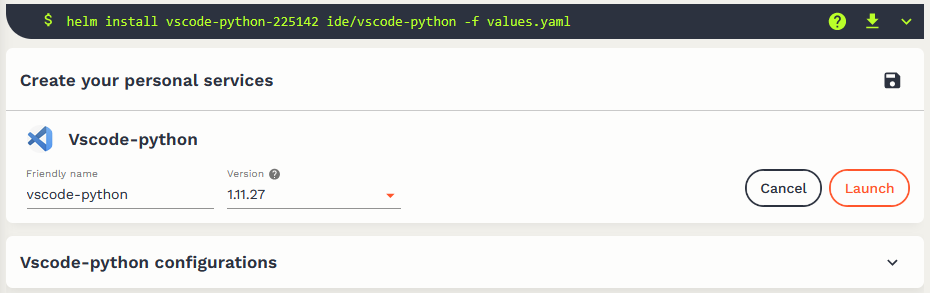
\includegraphics[width=\linewidth]{figures/service-configuration.png}
    \caption{Launching a service through Onyxia's UI.}
    \label{fig:service-configuration}
    \medskip
    {\footnotesize Note: Services from Onyxia's catalog can either be used vanilla or configured by the users to tailor them to their specific needs. In order to limit the dependence of users on Onyxia, each action performed by the user on the UI is accompanied by the actual command that is executed on the Kubernetes cluster.}
\end{figure}

Naturally, the way Onyxia makes statisticians more autonomous in their work depends on their needs and familiarity with IT skills. Statisticians that just want to have access to extensive computational resources to experiment with new data sources or statistical methods will have access in a few clicks to easy-to-use, pre-configured data science environments, so that they can directly start to experiment. However, many users want to go deeper and build actual prototypes of production applications for their projects: configuring initialization scripts to tailor the environments to their needs, deploying an interactive app that delivers data visualization to users of their choice, deploying other services than those available in our catalogs, etc. For these advanced users to continue to push the boundaries of innovation, Onyxia gives them access to the underlying Kubernetes cluster. This means that users can freely open a terminal on an interactive service and interacts with the cluster - within the boundaries of their namespace - in order to apply custom resources and deploy custom applications or services.

Besides autonomy and scalability, the architectural choices of Onyxia also foster reproducibility of statistical computations. In the paradigm of containers, the user must learn to deal with resources which are by nature ephemeral, since they only exist at the time of their actual mobilization. This fosters the adoption of development best practices, notably the separation of the code — put on an internal or open-source forge such as GitLab or GitHub — the data — stored on a specific storage solution, such as MinIO — and the computing environment. While this requires an entry cost for users, it also helps them to conceive their projects as pipelines, i.e. a series of sequential steps with well-defined inputs and outputs (akin to directed acyclic graph (DAG)). The projects developed in that manner are usually more reproducible and portable — they can work seamlessly on different computing environments — and thus also more readily shareable with peers.

\subsection{An extensive catalogue of services to cover the entire lifecycle of data science projects}
\label{ssec:catalog}

In developing the Onyxia platform, our intention was to provide statisticians with a comprehensive environment designed to support end-to-end development of data science projects. As depicted in Figure~\ref{fig:onyxia-catalog}, the platform offers a vast array of services that span the complete lifecycle of a data science project.

\begin{figure}[htbp]
    \centering
    \makebox[\textwidth][c]{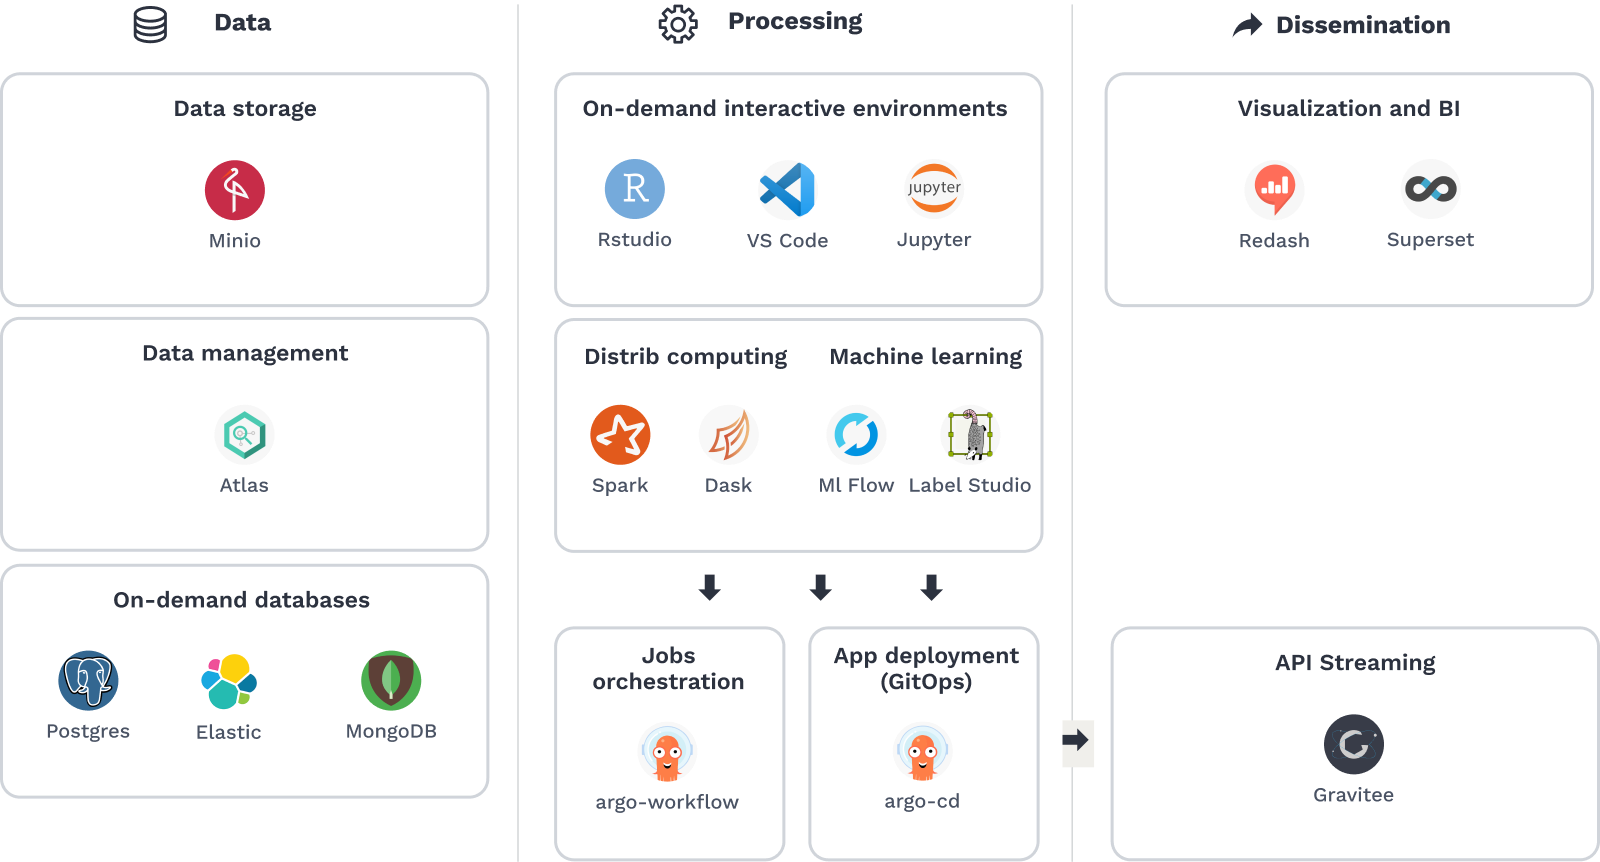
\includegraphics[width=1.2\textwidth]{figures/onyxia-catalog.png}}
    \caption{Onyxia's catalog aims at covering the entire lifecycle of data science projects}
    \label{fig:onyxia-catalog}
\end{figure}

The primary usage of the platform is the deployment of interactive development environments (IDE), such as RStudio, Jupyter, or VSCode. These IDEs come equipped with the latest kernels of major open-source programming languages commonly employed by public statisticians (R, Python, Julia), as well as an extensive collection of packages commonly used in data science for each language. In order to ensure that services remain up-to-date and consistent between them, we maintain our own stack of underlying Docker images and rebuild it weekly. The stack of images is fully open-source\footnote{\url{https://github.com/InseeFrLab/images-datascience}} and can thus be reused outside Onyxia.

As discussed in previous sections, the persistence layer of these interactive environments is mainly carried out by MinIO, Onyxia's default object storage solution. As it is based on a standardized REST API, files can be easily queried directly from R or Python using high-level packages. This in itself is an important step of ensuring reproducibility: the input files of a project are not mounted manually and then specified via paths adherent to a specific infrastructure and filesystem. Rather, files are specified as HTTP queries, making the overall structure of projects much more extendable. In our experience, the object-storage paradigm covers very well the needs of most statistical projects we accompany. However, additional database services such as PostgreSQL and MongoDB are available for applications with specific needs, such as those requiring online transaction processing (OLTP) capabilities or document-oriented storage.

As Onyxia was developed to allow experimentation with big data sources and machine learning methods, we also provide services optimized for scalability. For instance, frameworks like Spark and Trino that enable to perform distributed computations within Kubernetes. These services come pre-configured to integrate seamlessly with S3 storage, thus facilitating building integrated and efficient data pipelines.

Beyond mere experimentation, our goal is to empower statisticians to transition from trial phases to production-grade projects. In lines with principles from the DevOps approach, this involves facilitating the deployment of prototypes and their continuous improvement over time. To this end, we provide a set of open-source tools aimed at automatizing and industrializing the process of deploying data-intensive applications (ArgoCD, Argo-Workflows, MLflow). For projects leveraging machine-learning models, statisticians can serve their models through APIs, deploy them using the aforementioned tools, and manage their lifecycle using an API manager (e.g. Gravitee). Section~\ref{sec:mlops} will illustrate how these tools, particularly MLflow, have been central in putting machine learning models in production at Insee, in accordance with MLOps principles.

In section~\ref{ssec:principles}, we stressed that one of Onyxia's fundamental design principle was to avoid vendor lock-in. In line with this idea, organizations that implement Onyxia are free to customize catalogs to suit their specific requirements, or even opt to construct their own catalogs independent of Onyxia's default offerings. This flexibility ensures that organizations are not confined to a single solution or provider, and can adapt the platform to their evolving needs.

\subsection{Building commons: an open-source project and an open-innovation platform}

As a fully open-source initiative, the Onyxia project aims at building "knowledge commons" by promoting and building software that can be easily reused in official statistics and beyond \cite{schweik2006free}. This concerns, first of all, the components on which Onyxia are based: both its constitutive technological bricks (Kubernetes, MinIO, Vault) as well as all the services from the catalog are open-source. But more crucially, all the code of the project is available openly on GitHub\footnote{\url{https://github.com/InseeFrLab/onyxia}}. Alongside an in-depth documentation\footnote{\url{https://docs.onyxia.sh/}}, this greatly facilitates the potential for other organizations to create instances of data science platforms built upon the Onyxia software and tailor it to their respective needs (see figure~\ref{fig:onyxia-instances}). This enabled the project to attract a growing community of contributors from official statistics (Statistics Norway), NGOs (Mercator Ocean), research centres and even industry, thus transitioning progressively towards a more decentralized governance of the project. In the next years, the involvement of NSIs from the European Statistical System is expected to increase as Onyxia was chosen as the reference data science platform in the context of the AIML4OS project, a "One-Stop-Shop" for Artificial Intelligence/Machine Learning for Official Statistics in the European Statistical System.

\begin{figure}[htbp]
    \centering
    \makebox[\textwidth][c]{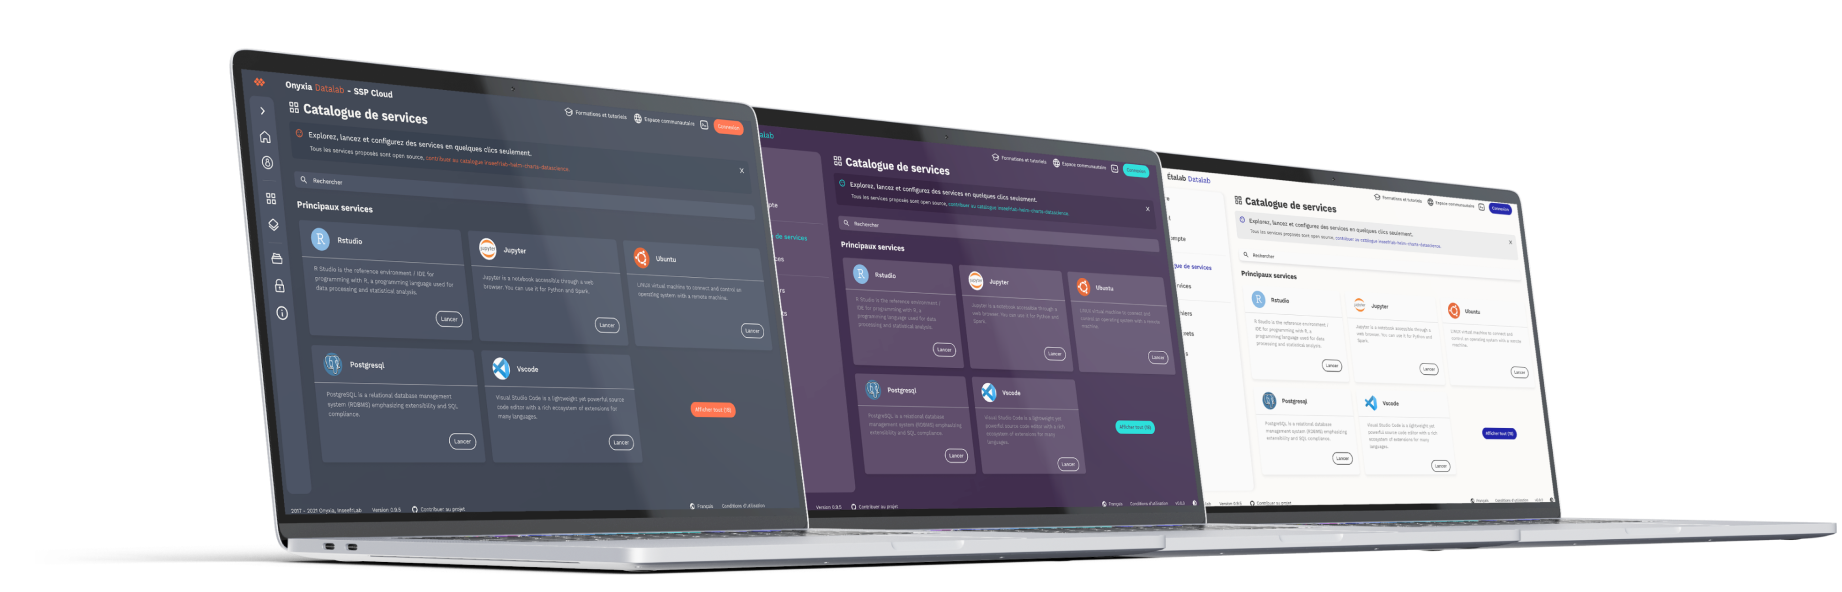
\includegraphics[width=1.3\textwidth]{figures/onyxia-instances.png}}
    \caption{One project, multiple instances: the UI is adaptable to the graphic identity of the organization}
    \label{fig:onyxia-instances}
\end{figure}

Another major way in which we try to build commons is by developing and maintaining a showcase instance of the Onyxia project, the SSP Cloud \cite{comte2022sspcloud}. This platform, equipped with extensive and scalable computational resources\footnote{On the physical side, the SSP Cloud consists in a Kubernetes cluster of about 20 servers, for a total capacity of 10 TB of RAM, 1100 CPUs, 34 GPUs and 150 TB of storage.}, is designed to be a sandbox for experimenting with cloud technologies and new data science methods. The full catalog of services of Onyxia is available on the platform, enabling motivated users to go beyond mere experimentation by producing "proof of concepts", with full autonomy regarding the configuration and orchestration of their services.

Beyond its technical capabilities, the SSP Cloud is an endeavour at embodying the principles of open-innovation \cite{chesbrough2003open}. Deployed on internet\footnote{\url{https://datalab.sspcloud.fr/}}, 
it is open not only to Insee employees, but also more broadly to all French governmental agencies and other European NSIs, and will serve as an official sandbox for the One-Stop-Shop program of the ESS described above. As a result, the platform is widely used in the French National Statistical System and even beyond, with about 800 unique users per month in 2024. These users form a dynamic community thanks to a centralized discussion canal; they help improve the user experience by reporting bugs, by suggesting new features, and by contributing directly to the project. The fundamentally collaborative nature of the SSP Cloud has proven especially beneficial for organizing innovative events such as hackathons — both at the national and international levels — and in the academic sphere. It has become an integral resource for several universities and Grandes Ecoles in France, fostering the use of cloud-native and reproducible environments, and preventing vendor lock-in effect due to the over-reliance of educational organizations on proprietary cloud solutions. Finally, the SSP Cloud plays a significant role in leveraging open data, particularly as it highlights and makes use of the growing abundance of datasets openly published by various statistical agencies.




\section{Case-study: using MLOps to improve NACE classification}
\label{sec:mlops}

This chapter aims, through a concrete example, to illustrate how Insee managed to deploy its first machine learning (ML) model into production. It provides an in-depth description of the MLOps approach that this project strived to adhere to, focusing on the various technologies that were employed. In particular, we highlight how cloud technologies were instrumental in building a solution iteratively and how Onyxia greatly facilitated this process by providing flexible development environments as well as tools to deploy and monitor models, promoting a continuous improvement loop. The entire project is available in open source\footnote{\url{https://github.com/orgs/InseeFrLab/teams/codification-ape/repositories}} and remains under active development.






\subsection{Improving the NACE classification process using ML methods}

\subsubsection{Motivation}

Coding tasks are common operations for NSOs and can sometimes be challenging due to the size of statistical classifications. At Insee, a sophisticated coding tool called Sicore was developed in the 1990s to perform various classification tasks \cite{meyer_sicore_1997}. It consists in a coding engine containing numerous deterministic rules which identify ground-truth labels. Each input label goes through these rules and when a ground-truth label is recognized, the associated code is assigned. When the label is not recognized, it must be manually classified by an Insee agent. 

Two main reasons drove the experimentation of new coding methods. 

Firstly, there was an internal change with the redesign of the French statistical business register, which lists all companies in France and assigns them a unique identifier used across public administrations. The main goals of this revamping were to improve the daily management of the registry for Insee agents and to reduce waiting times for companies. Additionally, at the national level, the government launched a one-stop shop for business formalities, allowing more flexibility for business owners in describing their main activities. Initial testing exercises revealed that Sicore was no longer the suitable tool for performing NACE classification, as only 30\% of the input data were being automatically coded.

Three stakeholders were involved in this project: the business team responsible for managing the French statistical business register, the IT team developing softwares related to the register's operation, and the innovation team responsible for implementing the new coding tool. The latter team is the SSP Lab, which was created in 2018 with the objective of providing support to other teams on innovation topics to streamline their various projects.

\subsubsection{Classification task}

The project we describe consists in a standard NLP classification problem. Starting from a textual description of the activity, we want to predict the associated class in the NACE Rev. 2 statistical classification. This classification has the particularity of being hierarchical and contains 5 different levels\footnote{Actually, there are 5 different levels in France but only 4 at the European level.}: section, division, group, class, and subclass. In total, 732 subclasses are included in the classification, which is the level at which we aim to perform the classification. Table \ref{tab:nace-nomenclature} provides an example of this hierarchical structure.

\begin{table}[htbp]
    \centering
    \begin{tabular}{llll}
    \textbf{Level} & \textbf{NACE} & \textbf{Title} & \textbf{Size} \\ \hline
    Section & H & Transportation and storage & 21 \\ \hline
    Division & 52 & Warehousing and support activities for transportation & 88 \\ \hline
    Group & 522 & Support activities for transportation & 272 \\ \hline
    Class & 5224 & Cargo handling & 615 \\ \hline
    \textbf{Subclass} & \textbf{\textcolor{red}{5224A}} & \textbf{Harbour handling} & \textbf{\textcolor{red}{732}} \\ 
    \end{tabular}
    \caption{NACE Nomenclature}
    \label{tab:nace-nomenclature}
    \end{table}

With the establishment of the one-stop shop, business owners now describe their activity description with a free-text field. As a result, the new labels are very different from the harmonized labels that were previously received. Therefore, it was decided to work with ML models, that are known to be effective on supervised text classification tasks \cite{li2022survey}. This represents a significant paradigm shift from Insee's perspective, as ML was not traditionally used in the actual production of official statistics. Besides, the perspective of putting the new model in production was considered from the outset, guiding numerous methodological and technical choices. As such, several strategic choices had to be made from the outset, including the methodology, the choice of a development environment consistent with the target production environment, and the adoption of collaborative work methods.

\subsubsection{Methodology}

Text classification from the free-text field provided by business owners is a complex task: the activity descriptions are relatively short and thus contain limited statistical information, can contain spelling mistakes, and often require domain knowledge to be properly classified. On such task, traditional text analysis methods such as count vectorization or TF-IDF often fall short whereas neural-network-based embedding methods tend to perform better \cite{li2022survey}. However, such architectures often impose greater computational demands, as they are much larger and might require specific hardware such as GPUs to perform inference with acceptable latency. These constraints led us away from the most powerful language models, such as Transformer models, and instead directed us towards the fastText model \cite{joulin2016bag}, a simpler embedding-based classifier. The fastText model is extremely fast to train, even from scratch, and inference does not require a GPU to achieve low latency time. Besides, the model yielded excellent performance results in our use-case that, considering the time and human resource constraints, were more than sufficient to enhance the existing process. Finally, the model's architecture is relatively simple, simplifying communication and adoption within the various Insee teams.

The fastText model relies on a bag-of-words model to obtain embeddings and a classification layer based on logistic regression. The bag-of-words approach involves representing a text as the set of vector representations of each of its constituent words. The specificity of the fastText model compared to other embeddings-based approaches is that embeddings are not only computed on words but also on word n-grams and character n-grams, providing more context and reducing biases due to spelling mistakes. Then, the embedding of a sentence is computed as a function of the individual token embeddings, typically the average. In the case of supervised text classification, the embedding matrix and the classifier's parameters are learned simultaneously during training by gradient descent, minimizing the cross-entropy loss function. Figure \ref{fig:fasttext} represents the full pipeline of operations performed by fastText on an example text input.

\begin{figure}[htbp]
    \centering
    \makebox[\textwidth][c]{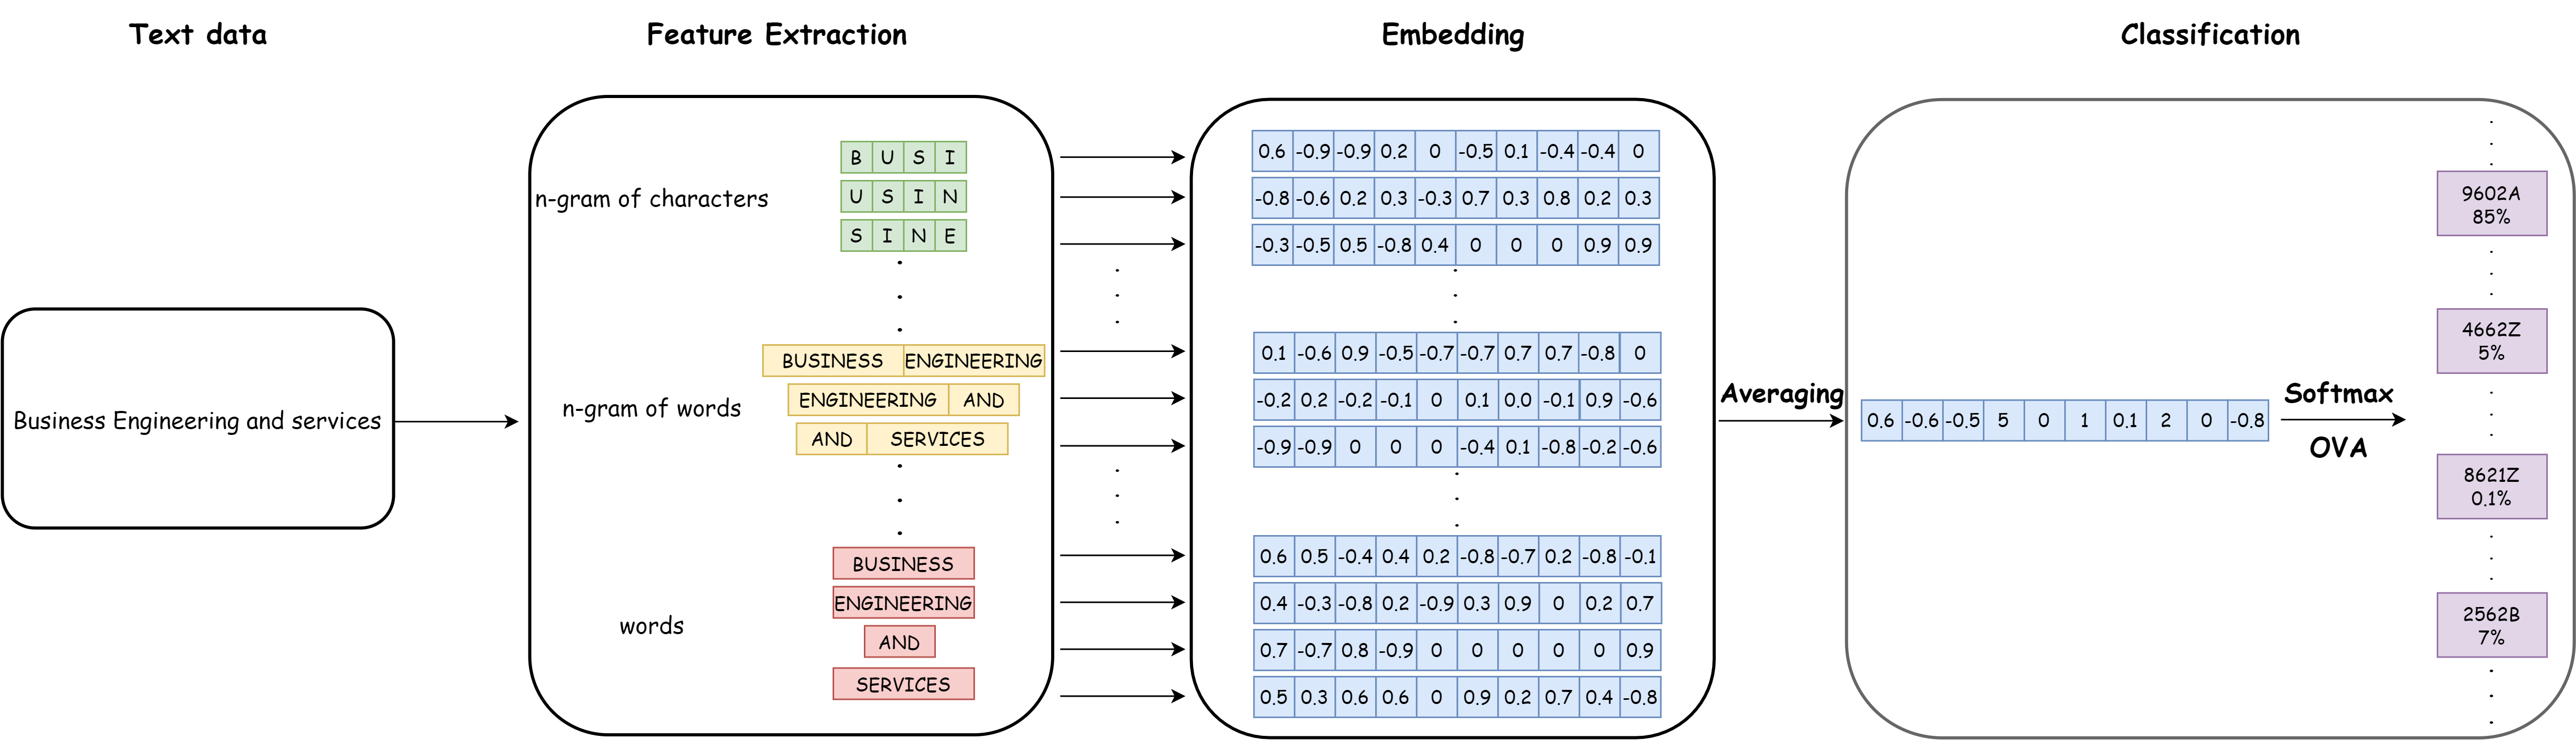
\includegraphics[width=1.5\textwidth]{figures/fasttext.png}}
    \caption{Overview of the simplified process behind fastText classifications}
    \label{fig:fasttext}
\end{figure}






\subsection{A production-first approach with MLOps}

From the very onset of this project, the target was to go beyond mere experimentation and put the model in production. Besides, the goal with this pilot project was also to build a template for future ML projects at Insee. We thus strove to enforce best development practices from the very beginning of the project: following community standards for code quality, using scripts-based development over notebooks, building a modular package-like structure, etc. However, compared to traditional development projects, machine learning projects have specific features that make it necessary to apply a complementary set of best practices, gathered under the name of MLOps.

\subsubsection{From DevOps to MLOps}
\label{subsubsec:devops-mlops}

DevOps is a set of practices designed to foster collaboration between development (Dev) and operations (Ops) teams. The fundamental idea is to integrate the full lifecycle of a project in a single automated continuum. An important tool to achieve this continuity is CI/CD pipelines. With continuous integration (CI), each commit of new source code will trigger a pipeline of standardized operations, such as building the application, testing it and making it available as a release. Then, continuous deployment (CD) consists in tools to automate the deployment of the new code and limit manual intervention, while ensuring proper monitoring to guarantee process stability and security. This approach promotes a faster, continual release of necessary feature changes or additions. Furthermore, by encouraging collaboration between teams, DevOps also promotes a quicker cycle of innovation, allowing teams to address issues as they arise and incorporate feedback effectively throughout the project lifecycle.

The MLOps approach can be seen as an extension of DevOps, developed to address the specific challenges related to managing the lifecycle of ML models. Fundamentally, both DevOps and MLOps aim at building software in a more automated and robust manner. The main difference is that in MLOps, this software also has a machine learning component. Consequently, the lifecycle of the project gets more complex. The underlying ML model needs to be re-trained regularly, to avoid any loss of performance over time. Data ingestion must also be included in the pipeline, as new data may be used to improve performance. Figure~\ref{fig:mlops-cycle} presents the steps of an ML project using the continuous representation traditionally seen in DevOps. This illustrates a fundamental principle of MLOps, the need for continuous improvement, described in more details in section~\ref{sec:principles-mlops}.

\begin{figure}[htbp]
    \centering
    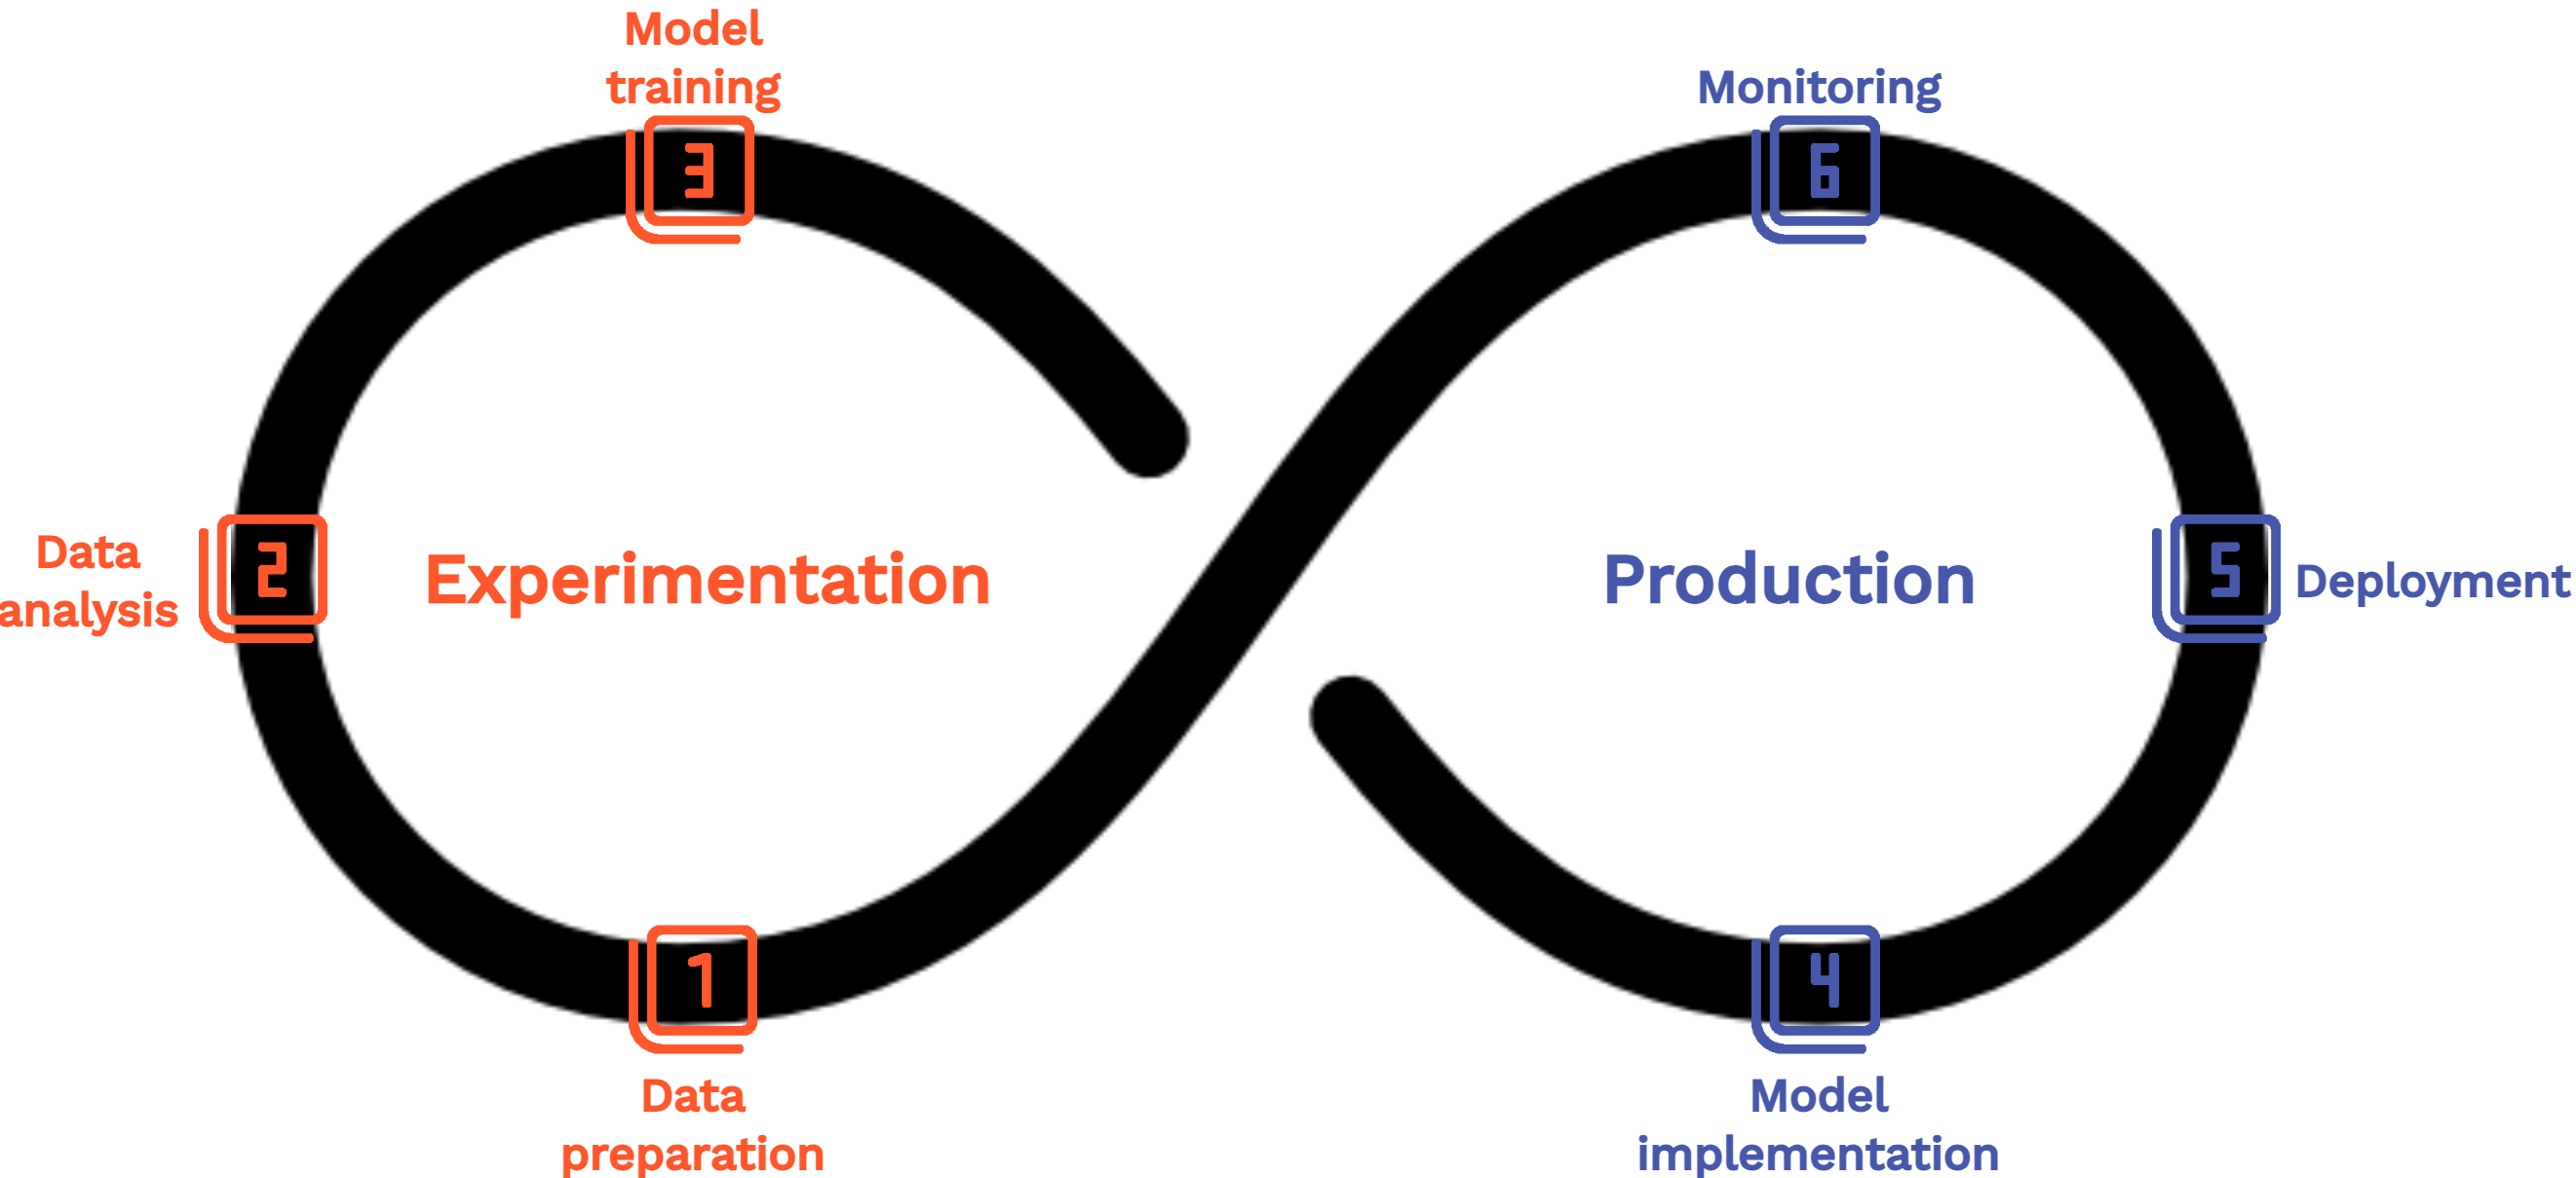
\includegraphics[width=\textwidth]{figures/mlops-cycle.png}
    \caption{The MLOps approach promotes a continuous management of ML projects lifecycle}
    \label{fig:mlops-cycle}
\end{figure}

\subsubsection{Principles of MLOps}
\label{sec:principles-mlops}

MLOps is defined by a few core principles that are crucial for building production-grade and scalable ML applications. These principles are designed to address the specific challenges associated with ML workflows.

The most fundamental principle of MLOps is continuous improvement, reflecting the iterative nature of ML projects. In the experimentation phase, the model is developed using a training dataset, that generally differs from the target data in some respect. When a model is deployed in production, the new data that the model needs to perform prediction on can reveal insights about the model's performance and potential shortcomings. These insights necessitate a return to the experimentation phase, where data scientists adjust or redesign their models to address any discovered issues or to improve accuracy. This principle thus emphasizes the importance of building a feedback loop that enables ongoing enhancements throughout the lifecycle of a model. Automation, particularly through the use of CI/CD pipelines, plays a crucial role in this process by making the transition between experimentation and production phases more continuous. Monitoring is also an essential part of this process: a model deployed in production needs to be continuously assessed so as to detect major drifts that may reduce the predictive performance of the model and thus necessitate further adjustments, such as re-training or fine-tuning the model.

Another major goal of MLOps is to promote reproducibility, ensuring that any ML experiment can be reliably reproduced with the same results. MLOps tools thus facilitate thorough logging of ML experiments, including data pre-processing steps, model hyperparameters, and training algorithms. Data, models, and code are versioned, enabling teams to revert to previous versions if an update does not perform as expected. Finally, these tools help to produce detailed specifications of the computing environment used to produce these experiments — such as versions of libraries — and often rely on containers to help replicate the same conditions in which the original model was developed.

Finally, MLOps aims at fostering collaborative work. ML-based projects generally involve a wider range of profiles: business units and data science teams on the one hand, developers and operations teams on the other. Like DevOps, MLOps thus emphasizes the need for a collaborative culture and to avoid working in silos. MLOps tools generally include collaborative features, such as centralized stores for ML models or ML features which facilitate the sharing of components between team members and limit redundancy.

\subsubsection{Implementation with MLflow}

Numerous tools have been developed to implement the MLOps approach in actual projects. All of these frameworks aim at enforcing, in some form, the core principles described above. In this project, we chose to rely on a popular open-source framework named MLflow\footnote{\url{https://github.com/MLflow/MLflow}}. This choice does not indicate any inherent superiority of MLflow over alternative software, but reflects a set of good properties associated with MLflow that made it a very relevant solution for our application. First, it covers the entire lifecycle of ML projects, while other tools may be more specialized in some parts of it. Second, it exhibits great interoperability as it is well-interfaced with popular ML libraries — such as PyTorch, Scikit-learn, XGBoost, etc. — and supports multiple programming languages — including Python, R, and Java, thus covering the spectrum of programming languages commonly used at Insee. Finally, it proved to be very user-friendly and thus encouraged adoption among the project members and facilitated continuous collaboration between them.

MLflow provides a cohesive framework to operationalize MLOps principles effectively within ML projects. Data scientists can encapsulate their work in MLflow Projects that package together ML code and its dependencies, ensuring that each project is reproducible and can be consistently re-executed. A project relies on an MLflow Model, a standard format that is compatible with most ML libraries and offers a normalized way of serving the model, e.g. via an API. This interoperability and standardization are instrumental in supporting continuous improvement of the project, as models trained with a variety of packages can be readily compared or switched by one another without breaking any code. As experiments with various models progress, the Tracking Server logs detailed information about each run — hyperparameters, metrics, and outputs artifacts and metrics — which there again promotes reproducibility but also facilitates the model selection phase through a user-friendly interface. After this experimentation phase, selected models are integrated into the Model Registry, where they are versioned and staged for deployment. This registry serves as a centralized model store that enables the different project members or teams to collaboratively manage the lifecycle of the project. Figure~\ref{fig:mlflow-components} shows the core components of MLflow and how they facilitate a more continuous and collaborative workflow inside an ML project.

\begin{figure}[htbp]
    \centering
    \makebox[\textwidth][c]{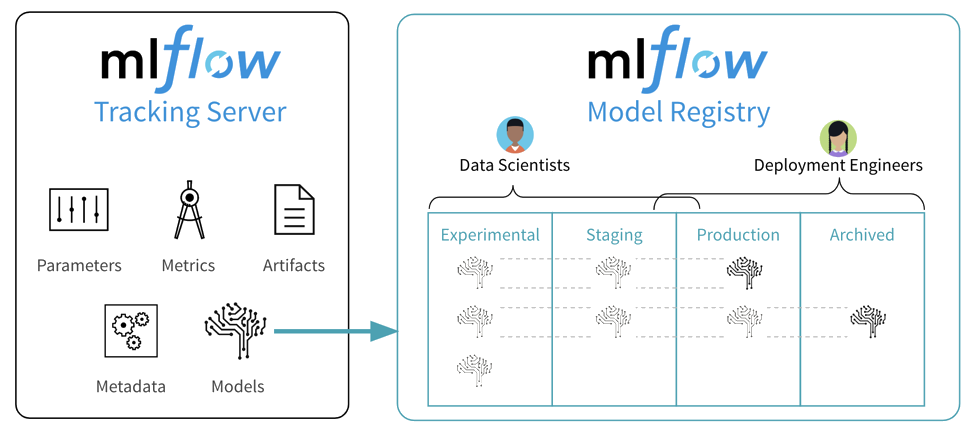
\includegraphics[width=\textwidth]{figures/mlflow-model-registry.png}}
    \caption{Core components of MLflow. Source: Databricks.}
    \label{fig:mlflow-components}
\end{figure}






\subsection{Facilitating iterative development with cloud technologies}

While continuous improvement is a fundamental principle of MLOps, it is also a very demanding one. In particular, it requires designing and building our project as an integrated pipeline whose various stages are mainly automated, from data ingestion to monitoring the model in production. In this context, iterative development is essential in order to build a minimum viable product that is then refined and improved over time. This section shows how cloud-native technologies, through the Onyxia project, were instrumental in building the project from the start as a collection of modular connected components, thus greatly enhancing the capacity for continuous refinement over time.

\subsubsection{A flexible development environment}

In a ML project, the flexibility of the development environment is essential. First, due to the diversity of tasks to be performed — data collection, preprocessing, modeling, evaluation, inference, monitoring, etc. Second, because ML is a fast-evolving field, it is preferable to build an ML app as a collection of modular components so as to be able to update components without disrupting the entire pipeline. As discussed in section~\ref{sec:cloud-native}, cloud-native technologies enable the creation of modular and scalable development environments.

However, as also discussed in section~\ref{sec:implementation}, access to such resources is not enough. An ML project requires a wide variety of tools to comply with MLOps principles — data storage, interactive development environments to experiment freely, automation tools, monitoring tools, etc. While these tools can be installed on a Kubernetes cluster, making them available to data scientists in an integrated and pre-configured manner is essential to facilitate their adoption. Through its catalog of services and the automatic injection of configuration in the services, Onyxia enables building projects that rely on multiple cloud-native components that can communicate readily with each other.

The way model training was carried out for this project emphasizes the flexibility provided by Onyxia in the experimentation phase. All the code performing the training is written in Python in the context of a VSCode service. As personal S3 credentials are injected in each service at startup, the various users of the projects can interact directly with the training data stored on a S3 bucket on MinIO, Onyxia's default object storage solution. All experiments performed for the model selection phase are logged on a shared instance of MLflow, which stores logged data on a PostgreSQL instance automatically launched on Kubernetes and artifacts (trained models and associated metadata) on MinIO. The model was trained using grid-search for hyperparameter tuning and evaluated through cross-validation, a combination that is known to provide a better evaluation of the generalization performance of the model but also requires a lot of computing resources, due to the combinatory nature of testing many hyperparameters combinations. In our case, we leveraged Argo Workflows, an open-source workflow engine designed to orchestrate parallel jobs on Kubernetes, each job being specified as an independent container. It then becomes straightforward to compare performances of the different trained models and select the best one using the comparison and visualization tools available in the UI of MLflow. 

In summary, the training stage was made efficient and reproducible thanks to the use of numerous modularly connected components — a distinctive feature of cloud-native technologies — readily made available to data scientists by Onyxia.

\subsubsection{Deploying a model}

Once candidate models have been optimized, evaluated and a best-performing model has been selected, the next step is to make it available to the application end users. Simply providing the trained model as an artifact or even just the code to train the model is not a convenient way to serve it, as it assumes that users have the resources, infrastructure, and knowledge required for training it under the same conditions. The goal is therefore to make the model available in a simple and interoperable manner, in the sense that it should be possible to query it with various programming languages. Furthermore, it should be possible for other applications to query the model in a programmatic way. 

Against that background, we opted to serve the model through a REST API. This technology has become a standard way to serve ML models as they offer several benefits. First, they fit very well a cloud-oriented environment: similarly to the other components of our stack, it makes it possible to query the model using standard HTTP requests, which contributes to the modularity of the system. It also means that they are interoperable: as they rely on standards technologies for queries (HTTP requests) and responses (generally, a JSON-formatted string), they are mostly agnostic to the programming language used to request them. Finally, they offer great scalability because of their stateless design\footnote{Stateless design refers to a system architecture where each request from a client to the server must contain all the information needed to understand and process the request. This means that the server does not store any information about the client's state between requests, allowing each request to be handled independently. This design simplifies scaling and enhances the robustness of the system, as any server can handle any request without relying on prior interactions.}. As each request must contain all the information needed to understand and process the request, REST APIs can easily be duplicated on different machines to balance a challenging load — a process known as horizontal scaling.

We developed the API serving the model with FastAPI\footnote{\url{https://fastapi.tiangolo.com}}, a fast and well-documented web framework for building APIs with Python. The API code and required software dependencies are encapsulated into a Docker image so that it can be deployed as a container on the Kubernetes cluster. An important benefit of using Kubernetes is the ability to scale the API — through the number of API pods effectively deployed — to the demand and provide automatic load-balancing. Upon startup, the API automatically retrieves the correct model from the MLflow model registry, which acts as a proxy from the actual artifact of the production model, stored on MinIO. Using a MLflow model enables to integrate the pre-processing step before each prediction to the API, greatly simplifying inference regardless of the ML framework used. This deployment process is summarized in Figure \ref{fig:api-datalab}.

\begin{figure}[htbp]
    \centering
    \makebox[\textwidth][c]{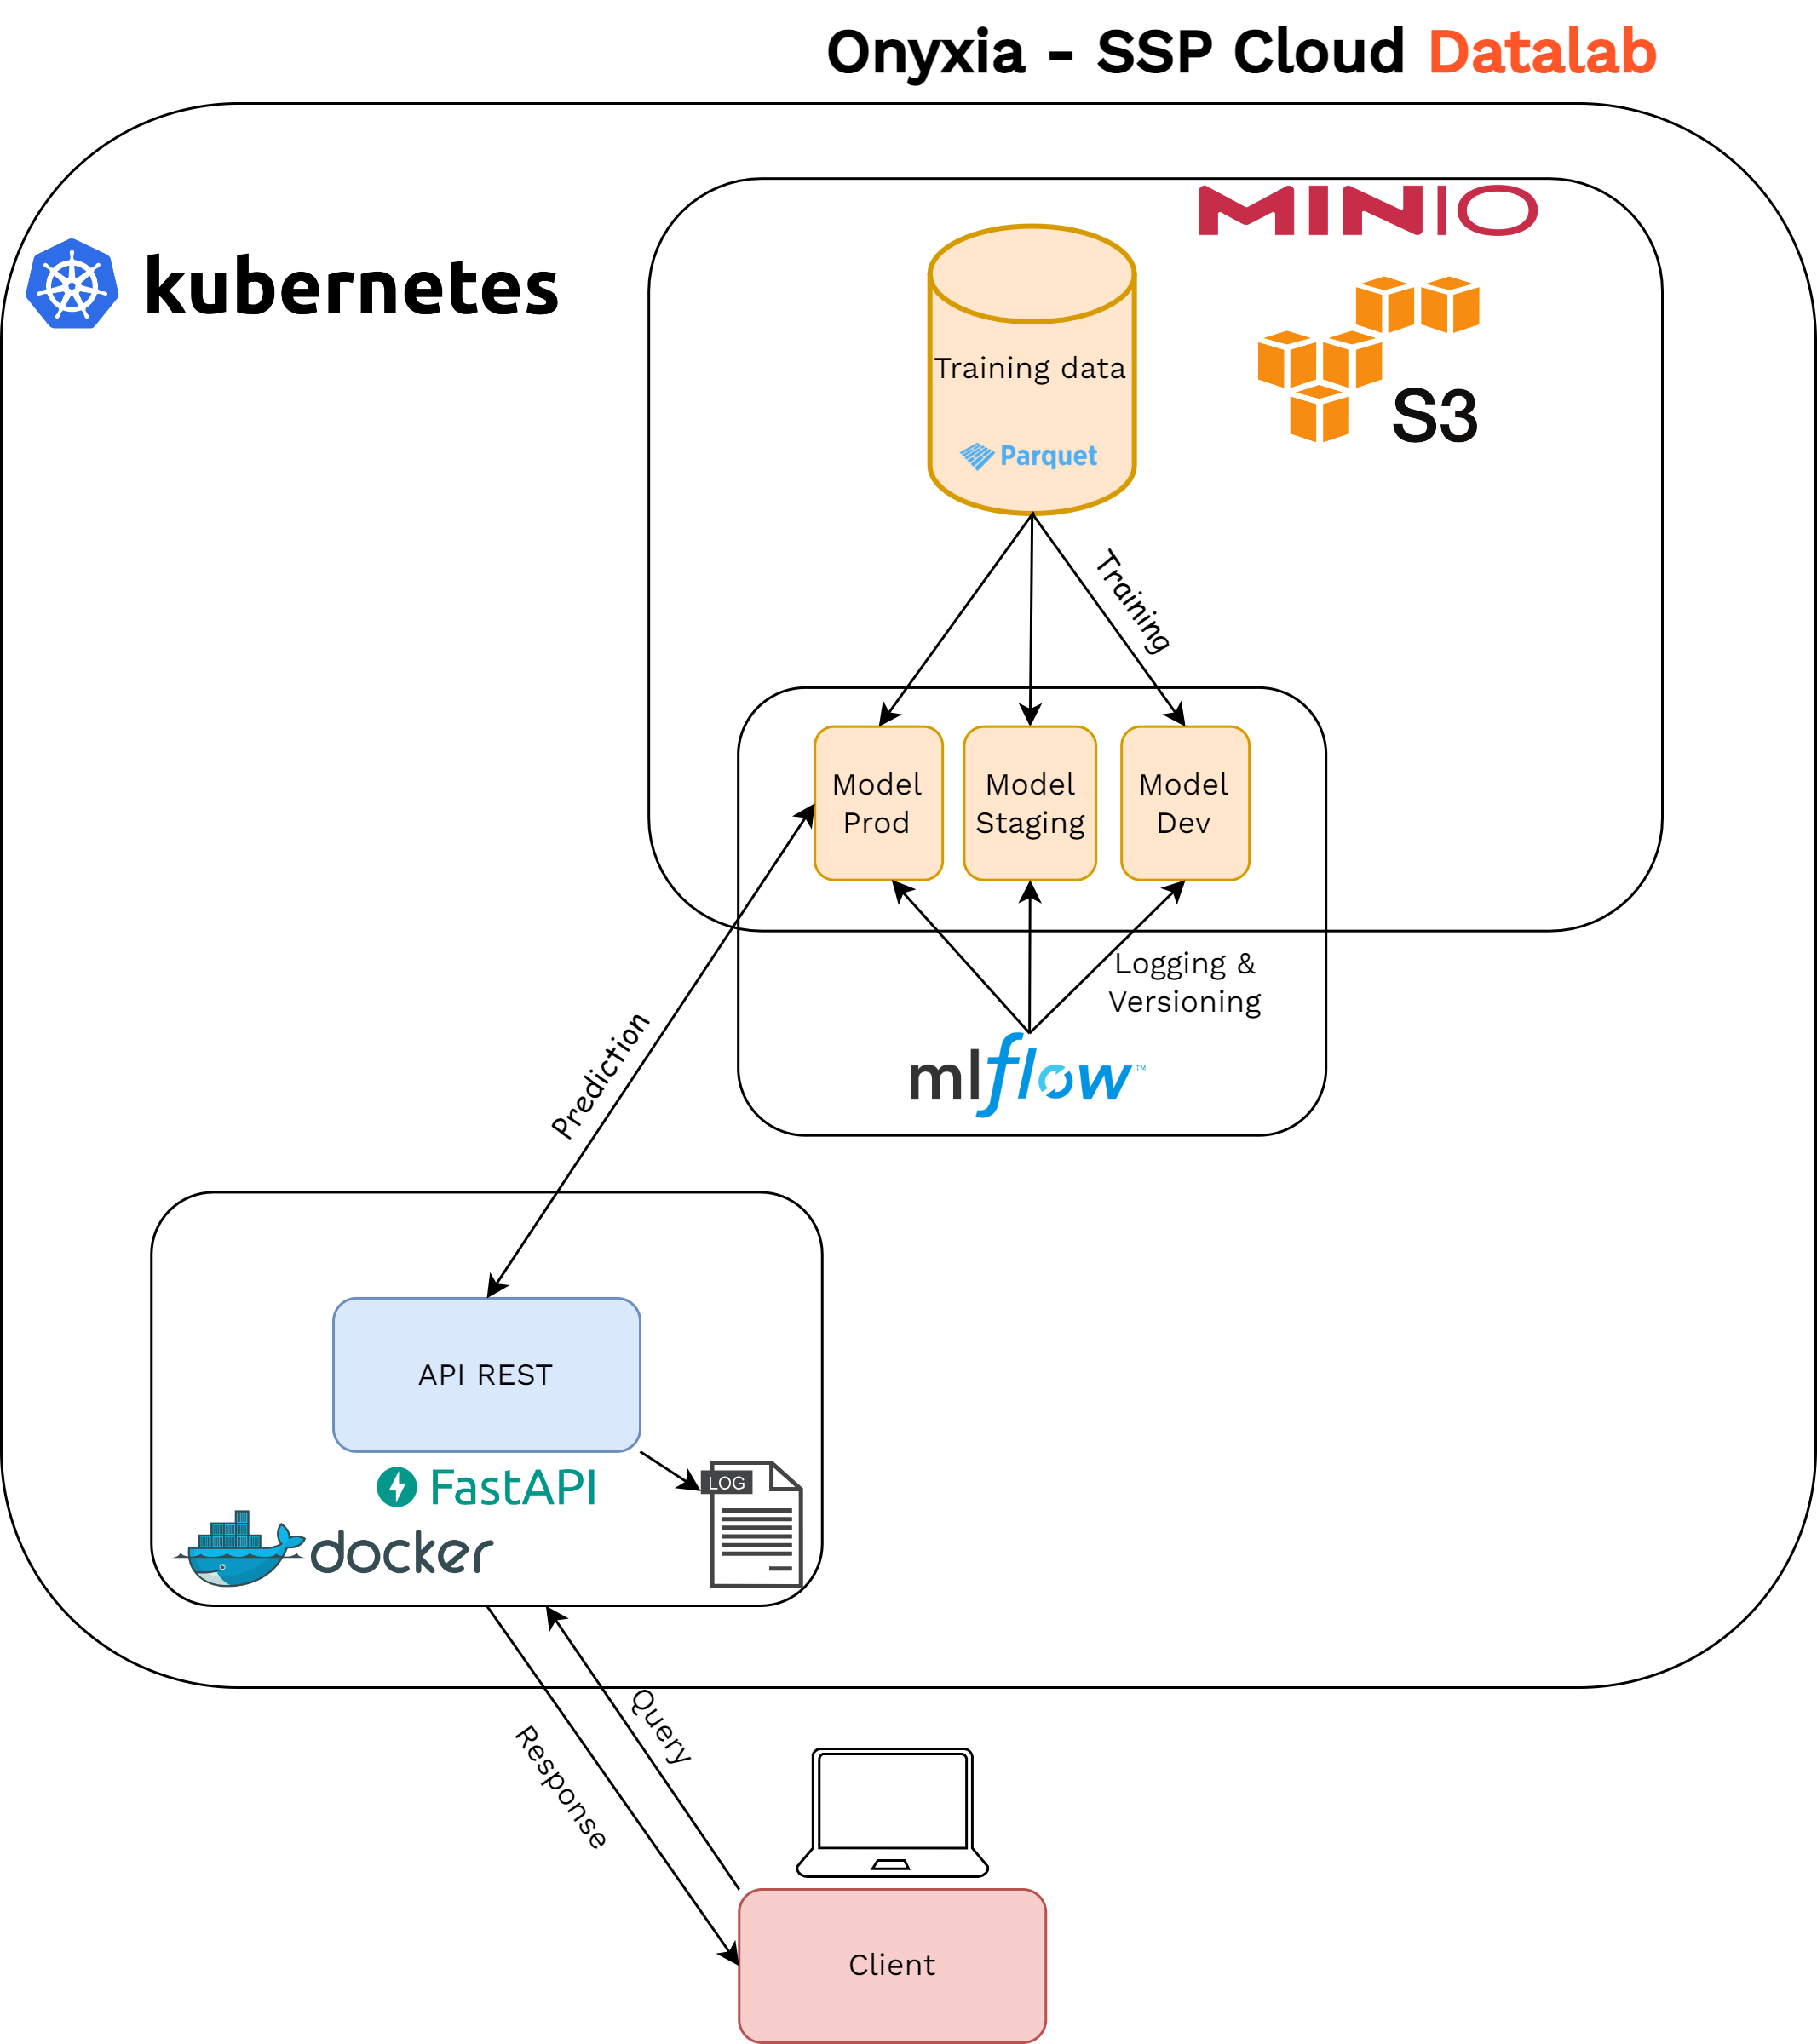
\includegraphics[width=0.75\textwidth]{figures/api-datalab.png}}
    \caption{A cloud-native approach to serve a ML Model using a REST API}
    \label{fig:api-datalab}
\end{figure}

\subsubsection{Building an integrated pipeline}

The architecture we built at this stage already reflects some important principles of MLOps. The use of containerization to deploy the API as well as the use of MLflow to track the experiments while developing the model ensures reproducibility of the predictions. Using the central model registry provided by MLflow facilitates the management of the lifecycle of the models in a collaborative way. Furthermore, the modularity of our architecture leaves room for further improvement as modular components can be easily added or modified without breaking the structure of the application as a whole. As we shall see in subsequent sections, this property was essential in building the application iteratively, enabling to add a monitoring layer (Section~\ref{subsubsec:monitoring}) and an annotation component (Section~\ref{subsubsec:annotation}) to promote continuous improvement of the model.

However, the ability to refine the base architecture iteratively also requires more continuity in the process. At this stage, the deployment process involves several manual operations. For instance, adding a new feature to the API would require to build a new image, tag it, update the Kubernetes manifests used to deploy the API and enforce them on the cluster to replace the existing one with minimum downtime. Similarly, a change of the model served through the API would require a very simple modification of the code but several manual steps to update the version on the cluster. As a result, data scientists are not fully autonomous when it comes to prototyping and testing updated versions of the model or the API, which limit the potential for continuous improvement.

In order to automate this process, we built a CI/CD pipeline — a concept already presented in Section~\ref{subsubsec:devops-mlops} — integrating these various steps. Figure \ref{fig:ci-cd} illustrates our specific implementation of a CI/CD pipeline. Any change in the code of the API repository triggers a CI build process (implemented with GitHub Actions) of the associated docker image, which is then released on a public container registry (DockerHub). This image can then be fetched and deployed by the container orchestrator (Kubernetes), by specifying and applying manually new manifests to update the Kubernetes resources of the API. However, the downside of this approach is that it limits reproducibility of the deployment, since each resource is handled independently by the orchestrator, so that the lifecycle of the API deployment as a whole is not managed. To overcome this shortcoming, we integrate the deployment part in a CD pipeline based on the GitOps approach: the resources manifest of the API are stored on a Git repository. The state of this "GitOps" repository is monitored by a Kubernetes operator (ArgoCD), so that any change in the application manifests is directly propagated to the deployment on the cluster. In this integrated pipeline, the only action needed for the data scientist to trigger an update of the API is to change the tag of the API image indicating the version to be deployed.

\begin{figure}[htbp]
    \centering
    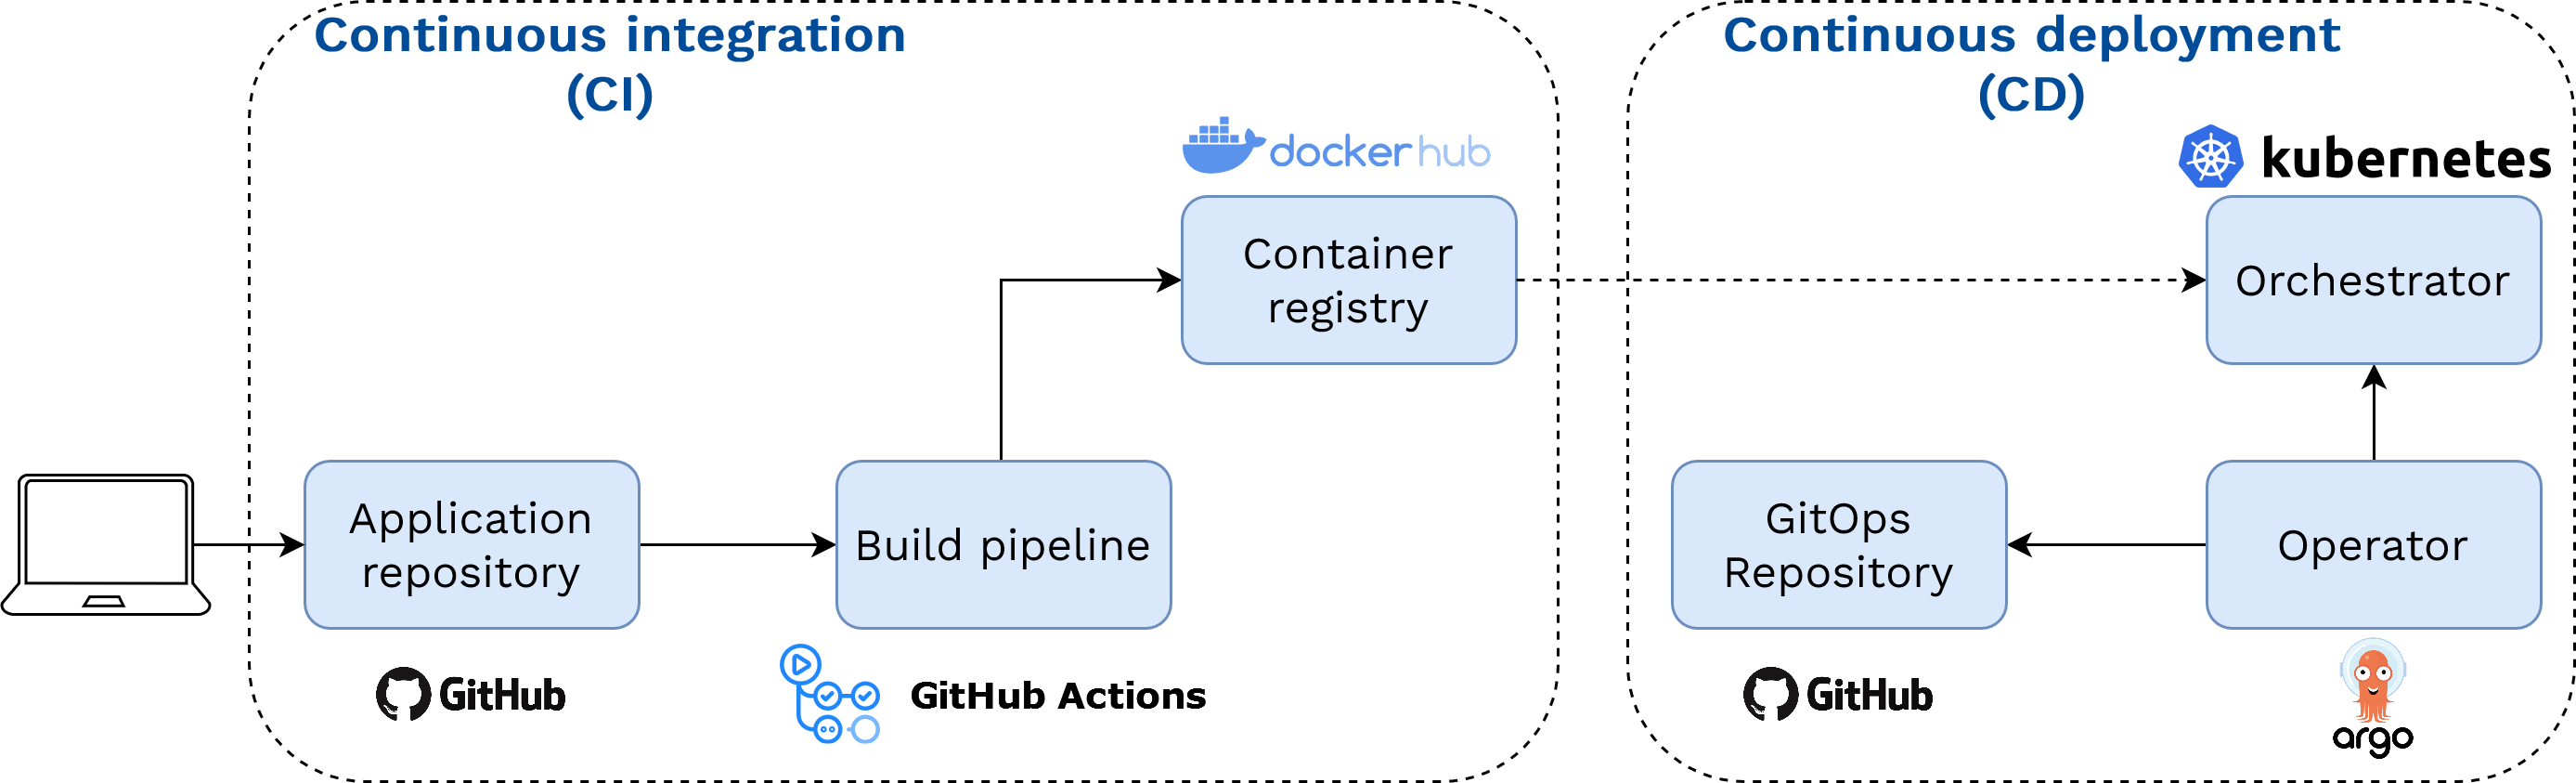
\includegraphics[width=\textwidth]{figures/ci-cd.png}
    \caption{The CI/CD pipeline implemented in the project}
    \label{fig:ci-cd}
\end{figure}

\subsubsection{Monitoring a model in production}
\label{subsubsec:monitoring}

Once the initial development phase of the project has been completed — including training, optimization, and deployment of the model to be served to users — it is crucial to understand that the data scientist's responsibilities extend further. Traditionally, the role of the data scientist is often limited to training the model and selecting the model to deploy, with the deployment task being delegated to the IT department. However, a specificity of ML projects is that, once in production, the model has not yet reached the end of its lifecycle, and it must be continuously monitored to prevent undesirable performance degradation. Continuous monitoring of the deployed model is extremely important to ensure the conformity of results to expectations, anticipate changes in data, and iteratively improve the model.

The concept of monitoring can take on different meanings depending on the context of the involved team. For IT teams, it primarily involves verifying the technical effectiveness of the application, including aspects such as latency, memory consumption, or disk usage. Conversely, for data scientists or business teams, the focus is more on methodological monitoring of the model. However, real-time tracking of the performance of an ML model is often a complex task, given that ground truth is usually not known at the time of prediction. Therefore, it is common to use proxies to detect any signs of performance degradation. Two main types of degradation of an ML model are generally distinguished. The first one is data drifts, which occur when the data used during inference in production exhibits significant differences compared to the data used during training. The second one is concept drifts, which occur when a change in the statistical relationship between the features and the target variable is observed over time.

In the context of our project, the objective is to achieve the highest rate of correctly classified textual description while minimizing the number of textual description requiring manual intervention. Thus, our goal is to distinguish correct predictions from incorrect ones without prior access to ground truth. To accomplish this, we use a confidence index defined as the difference between the two highest confidence scores of the top results returned by the model. For a given textual description, if the confidence index exceeds a determined threshold, the textual description is automatically coded. Otherwise, the textual description is manually coded by an Insee agent. This manual coding task is still informed by the ML model: through an application that queries the API, the agent is shown the five most probable codes according to the model. 

Defining the threshold for automatic coding of textual descriptions was thus crucial in this process, and involved making a trade-off between achieving a high automatic coding rate and maximizing coding performance. To monitor the behaviour of our model in production, we developed an interactive dashboard that enables visualization of several metrics of interest for the business teams. Among these metrics are the number of requests per day and the rate of automatic coding per day based on a given confidence index threshold. This visualization allows business teams to understand the rate of automatic coding they would have obtained if they had chosen different thresholds. This dashboard also represents the distribution of obtained confidence indices and compare temporal windows in order to check for changes in the distributions of predictions returned by the model\footnote{Such distribution changes are typically checked by computing statistical distances — such as the Bhattacharyya distance, the Kullback-Leibler divergence, the Hellinger distance — and/or by performing statistical tests — such as the Kolmogorov–Smirnov or the chi-squared test.}. Finally, confidence indices can be analysed at finer levels of granularity based on the aggregation level of the statistical classification, to determine which classes are most difficult to predict and which have more or less occurrences.

Figure \ref{fig:full-architecture} shows the components that were added to the project architecture so as to provide the monitoring dashboard described above. First, we set up a simple Extract-Transform-Load (ETL) process in Python (second box of the bottom row), which fetches the API logs periodically and transforms them into partitioned Parquet files\footnote{Ideally, existing frameworks should be preferred over custom-made solutions to prioritize standardized routines. At the time of building this component of the pipeline, we found that existing, cloud-native frameworks for log analytics had important limitations. This constitutes an area of improvement for the project.}. Then, we use the Quarto framework\footnote{Successor to R Markdown, Quarto has become an essential tool of our data stack. It unifies the functionality of several very useful packages from the R Markdown ecosystem while providing native support of several programming languages, including Python and Julia in addition to R. It is increasingly used at Insee as a way to produce reproducible documents and output them in a variety of formats.} to build an interactive dashboard (third box of the bottom row). To compute the various metrics presented in the dashboard, the Parquet files are queried using the SQL language through the DuckDB engine. Like the API, the dashboard is built and deployed as a container on the Kubernetes cluster, and this process is automated using a CI/CD pipeline. The annotation component (fourth box of the bottom row) is discussed in the next section.

\begin{figure}[htbp]
    \centering
    \makebox[\textwidth][c]{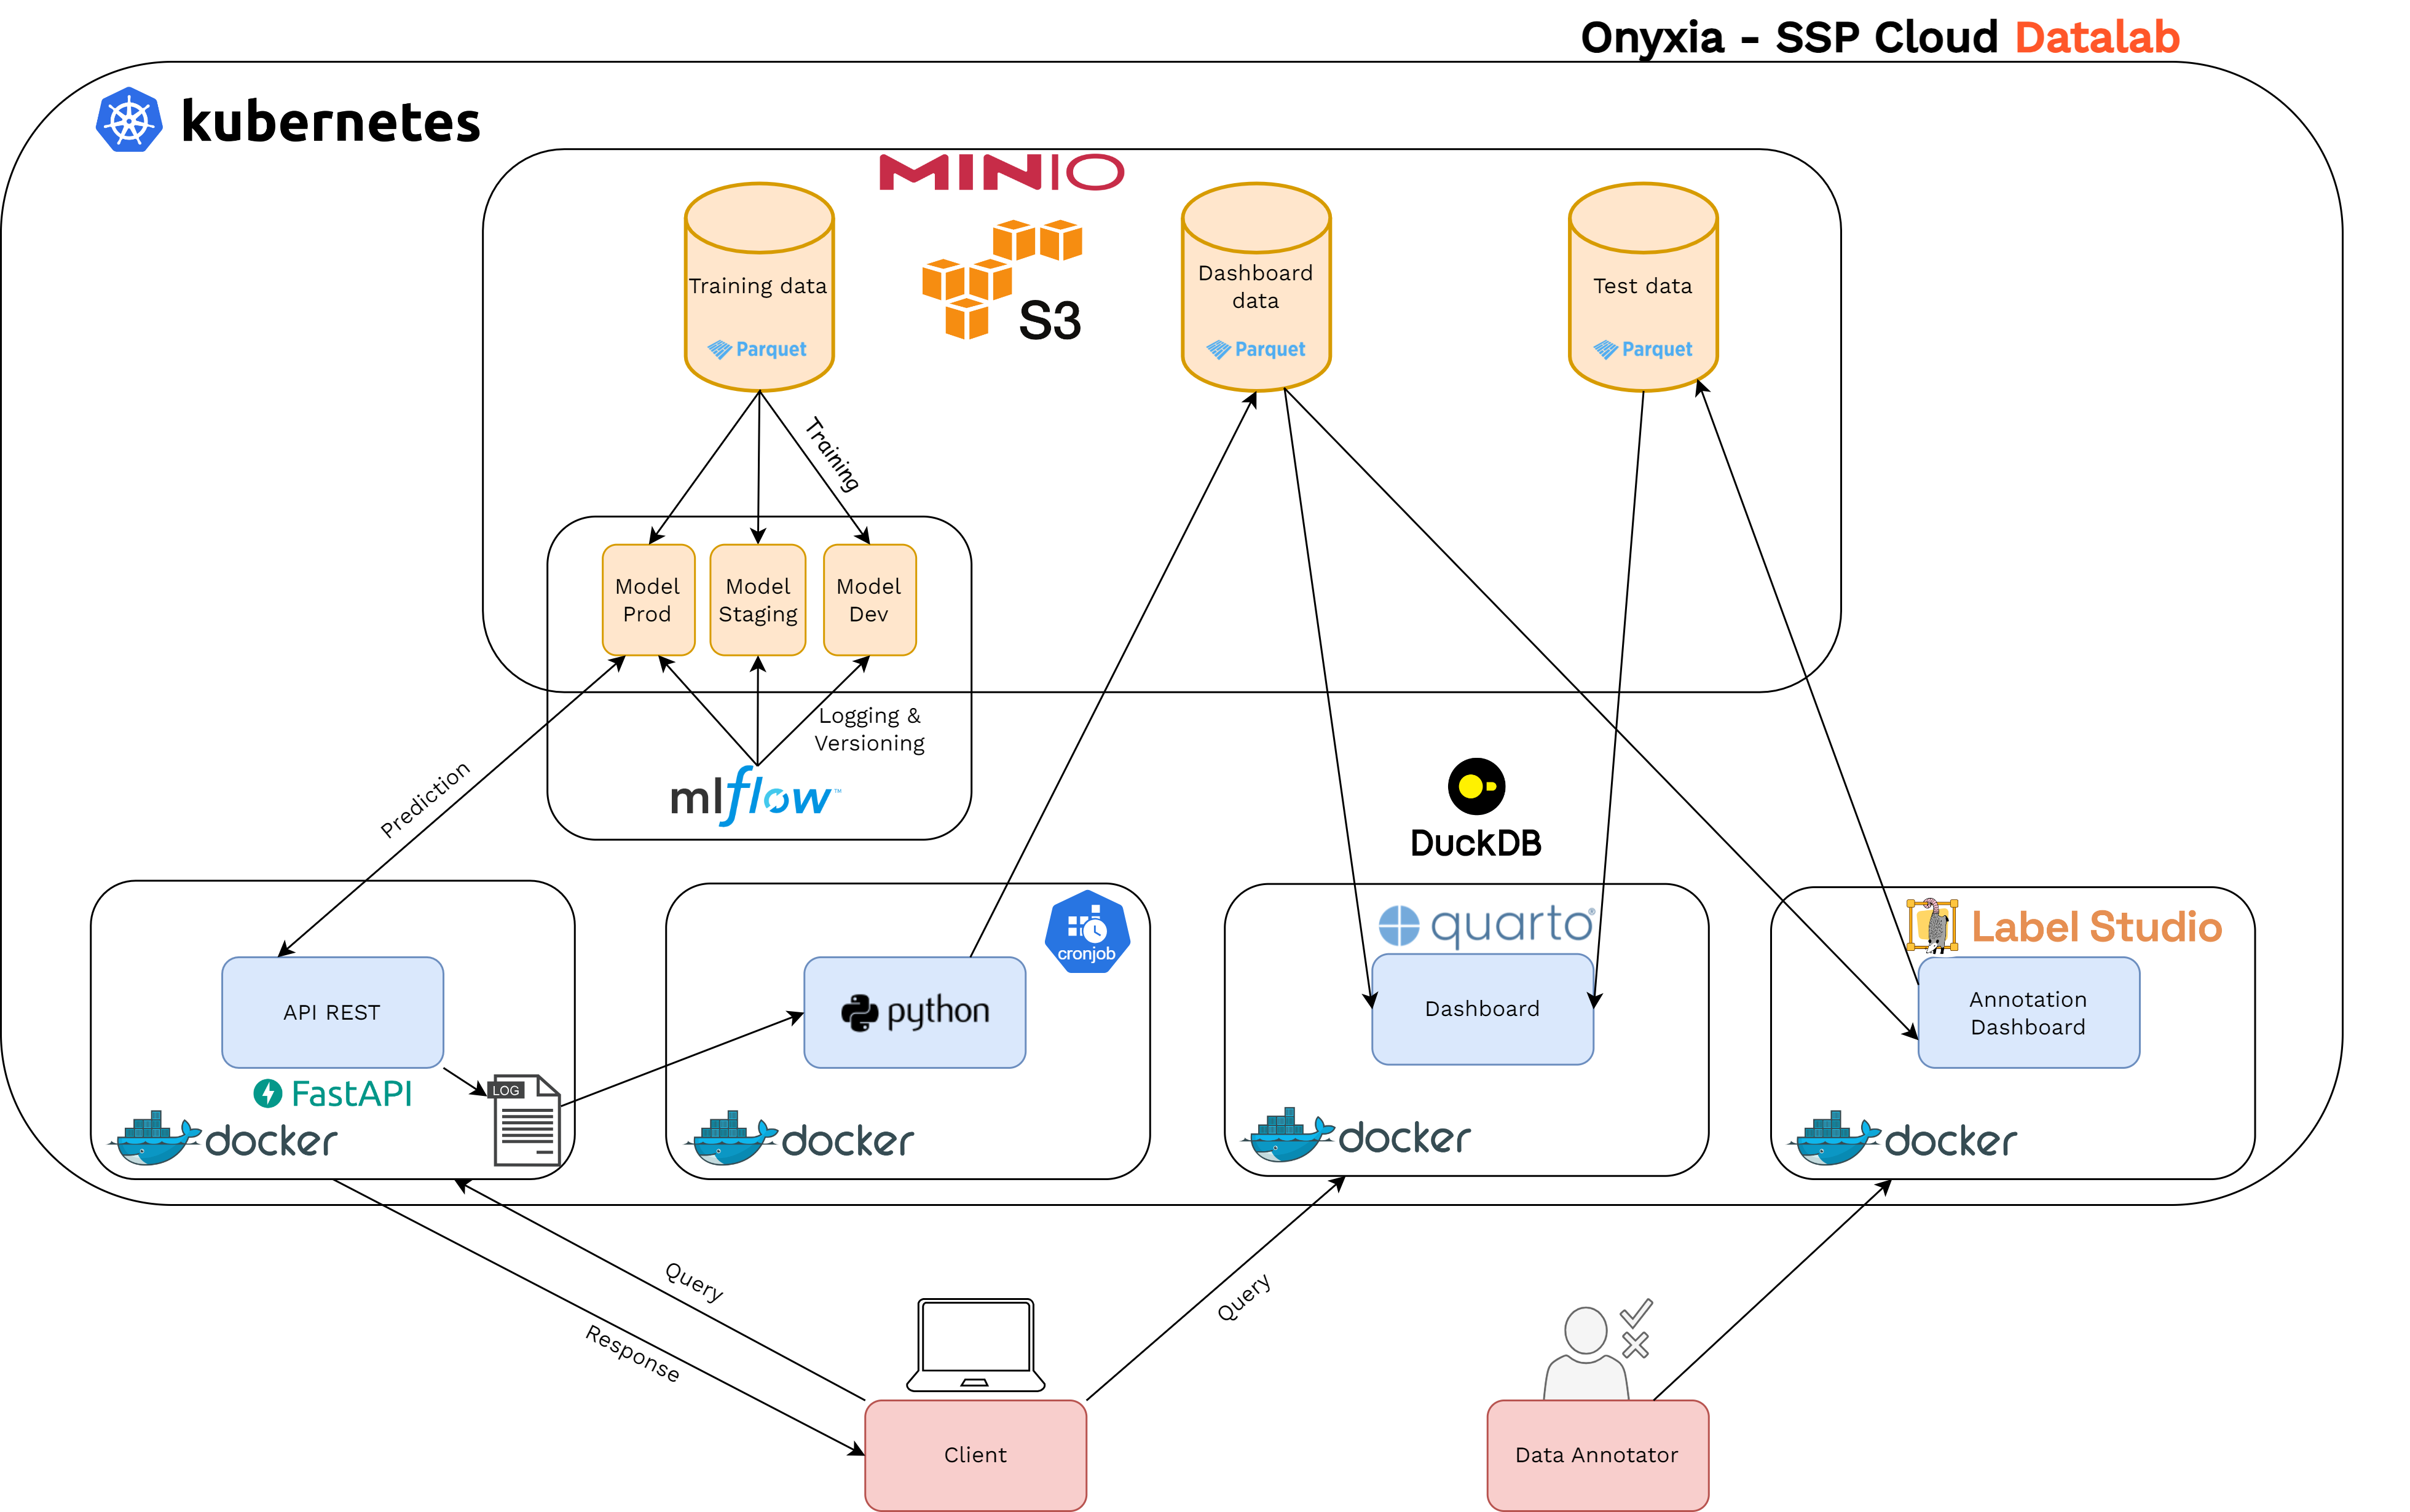
\includegraphics[width=1.5\textwidth]{figures/annotation-datalab.png}}
    \caption{Our implementation of a complete MLOps architecture}
    \label{fig:full-architecture}
\end{figure}

\subsubsection{Promoting continuous improvement of the model}
\label{subsubsec:annotation}

The monitoring layer of our application provides an important and detailed view into the system performance. Due to the dynamic nature of real-life data, ML models' performance often declines over time. To promote continuous improvement of the model, it is thus essential to envision strategies to overcome these performance losses. A frequently used strategy is periodic re-training of the model, requiring the collection of new training data.

Several months after the first version of the model was deployed in production, the need to implement a continuous annotation process became increasingly apparent for two key reasons. First, a gold-standard sample was not accessible at the time of the experimentation phase, so we relied on a subset of the training dataset to perform evaluation, knowing the labeling quality was not optimal. Continuously collecting a gold-standard sample would thus enable us to get an unbiased view of the model's performance in production on real data, particularly on data that has been automatically coded. Another reason is the redesign of the NACE statistical classification in 2025. From 2025 onwards, NSOs will be required to use the latest version of NACE, namely NACE Rev. 2.1. This revision brings substantial changes that will require an adaptation of the model, and thus the collection of new training set. Annotation of the old training dataset according to the new statistical classification will be necessary.

Against that background, an annotation campaign has been initiated in early 2024 to continuously build a gold-standard dataset. The annotation campaign is carried out on the SSP Cloud using Label Studio, an open-source annotation tool that provides a user-friendly interface and is available in Onyxia's catalog. Figure \ref{fig:full-architecture} illustrates how the labelling component (fourth box of the bottom row) could be readily integrated in the project architecture thanks to its modular nature. In practice, we create a pool of text descriptions randomly sampled from the data passed through the API over the past three months. This sample is then sent to annotation by NACE experts using the UI of Label Studio. The annotation results are automatically saved on MinIO, transformed into Parquet format. Then, these gold-standard data are directly integrated into the monitoring dashboard to compute and observe various model performance metrics. These metrics give us a much clearer picture on the actual performance of the model on production data, and in particular on its shortcomings. In parallel, we will launch an annotation campaign in the upcoming months to construct a new training set tailored to the recently updated NACE statistical classification. Leveraging both the updated training data and performance metrics derived from the gold-standard sample, we aim to iteratively enhance the model's accuracy through periodical and targeted re-training in the near future.


\section{Discussion}

The development of data science methods offers considerable potential for official statistics. However, our ability to create value from these new methods essentially depends on our capacity to produce production-grade systems that serve their purpose in a robust way. This evolution calls for deep reflection on what constitutes a modern, scalable data science infrastructure for official statistics. This article presents the Onyxia project, the proposal for such a platform that we are developing at Insee. By exploiting cloud-native technologies that have become standards in the data eco-system, it aims to increase statisticians' autonomy in the orchestration of their statistical treatments, while promoting reproducibility of produced statistics. As cloud technologies are notoriously difficult to configure, the core value of Onyxia's lies in making them accessible to statisticians via a user-friendly interface and a catalog of pre-configured services to cover most common uses. Through an internal project aiming at revising the NACE classification process using machine learning methods, we illustrate how Onyxia enables to iteratively build production-grade machine learning projects that promote continuous improvement, a fundamental principle of the MLOps approach.

Initially developed as an internal project, Onyxia has gained recognition beyond the scope of Insee or the French administration. Convinced of the potential of cloud technologies to foster autonomy and leverage the full potential of data science, several organizations now have a production instance of Onyxia running, and multiple others are in the process of either testing or implementing one. Besides, the choice of Onyxia as the reference data science platform in the context of the AIML4OS project should further facilitate its adoption within the ESS. This trend is naturally very beneficial to the Onyxia project, as it moves from a project developed in open-source — but mainly at Insee — to a full open-source project with a growing base of contributors. This in turn facilitates its adoption by other organizations, since it gives more guarantees on its sustainability independently of Insee's strategy. The governance of the project is currently evolving to reflect this trend. For instance with the organization of monthly community calls and the creation of a public channel and roadmap for the project\footnote{All information are available on the GitHub depository of the project: \url{https://github.com/InseeFrLab/onyxia}}.

Despite this success, we observe several limitations to the widespread adoption of the project in organizations. First, it is essential to remind that the fundamental choice made by organizations that adopt Onyxia is not the software itself, but the underlying technologies: containerization (through Kubernetes) and object storage. These technologies can represent substantial entry costs for organizations, as they demand a significant commitment to developing and maintaining skills which are not readily found in NSOs. Yet, the general trend towards cloud-native solutions among data-centric organizations suggests a favourable shift that could mitigate these challenges over time.

Similarly, the transition towards cloud-native technologies induces entry costs for statisticians. First, they often deal with a loss of references regarding where computations actually happen: while they may be accustomed to performing computation on centralized servers rather than a personal computer, the container adds a layer of abstraction that make the location hard to grasp at first. But the major perceived change in this paradigm is the loss of data persistence. In traditional setups — either a personal computer or a server accessed through a virtual desktop — the code, the data and the computing environment are kind of mixed in a black box fashion. On the contrary, containers have no persistence by design. While object storage provides this persistence, a proper use of these infrastructures for statistical projects require a variety of tools and corresponding skills: using a version control system for the code, interacting with the object storage API to store the data, providing configuration files or secrets as inputs, etc. In a way, these entry costs can be seen as the "price" of autonomy: thanks to cloud-native technologies, statisticians now have access to scalable and flexible environments that enable them to experiment more freely, but this autonomy requires a significant skills upgrade which may be overwhelming at first and limit adoption. However, our experience at Insee suggests that this effect can largely be mitigated through a combination of training statisticians to development best practices and accompanying statistical projects when transitioning to cloud infrastructures.

While Onyxia has significantly democratized access to cloud-native technologies for statisticians, the actual integration of data science methods in the statistical production of NSOs encompasses broader challenges, organizational in nature. A major hindsight from the deployment of our first ML model in production is the necessity to overcome skill compartmentalization across IT, business, and innovation teams. By nature, production-grade ML projects involve a wide range of skills — knowledge of the business domain, model training and fine-tuning, deployment and monitoring — and thus effective collaboration between professionals with different work cultures, programming languages, etc. Our experience shows that cloud technologies, by fostering autonomy of data scientists, give more continuity to ML projects and facilitate this much needed collaboration between various profiles. However, fully addressing these challenges involve measures that go beyond the technical domain. For instance, embedding some data science capabilities directly within business teams, in complement of centralized innovation teams, could foster better alignment with project objectives. Also, recruiting profiles that are not typically present in NSOs, such as data engineers or ML engineers, could bring new essential skills that lie at the intersection of statistical methodology and computer techniques. Ultimately, the transition towards a data science-driven approach in statistical production should rely on a balanced strategy that couples technical solutions such as Onyxia with comprehensive organizational adjustments, fostering a culture of collaboration, continuous learning, and innovation.

\bibliographystyle{plain}
\bibliography{references}

\end{document}
